%%%%%%%%%%%%%%%%%%%%%%%%%%%%%%%%%%%%%%%%%
% Journal Article
% LaTeX Template
% Version 2.0 (February 7, 2023)
%
% This template originates from:
% https://www.LaTeXTemplates.com
%
% Author:
% Vel (vel@latextemplates.com)
%
% License:
% CC BY-NC-SA 4.0 (https://creativecommons.org/licenses/by-nc-sa/4.0/)
%
% NOTE: The bibliography needs to be compiled using the biber engine.
%
%%%%%%%%%%%%%%%%%%%%%%%%%%%%%%%%%%%%%%%%%

%----------------------------------------------------------------------------------------
%	PACKAGES AND OTHER DOCUMENT CONFIGURATIONS
%----------------------------------------------------------------------------------------

\documentclass[
	a4paper, % Paper size, use either a4paper or letterpaper
	10pt, % Default font size, can also use 11pt or 12pt, although this is not recommended
	unnumberedsections, % Comment to enable section numbering
	twoside, % Two side traditional mode where headers and footers change between odd and even pages, comment this option to make them fixed
]{LTJournalArticle}


\usepackage{float}
\usepackage{graphicx}
\usepackage{longtable}
\usepackage{supertabular,booktabs}
\usepackage{tikz}
\def\checkmark{\tikz\fill[scale=0.4](0,.35) -- (.25,0) -- (1,.7) -- (.25,.15) -- cycle;} 

%\addbibresource{sample.bib} % BibLaTeX bibliography file




%\runninghead{Shortened Running Article Title} % A shortened article title to appear in the running head, leave this command empty for no running head

%\footertext{\textit{Journal of Biological Sampling} (2024) 12:533-684} % Text to appear in the footer, leave this command empty for no footer text

\setcounter{page}{1} % The page number of the first page, set this to a higher number if the article is to be part of an issue or larger work

%----------------------------------------------------------------------------------------
%	TITLE SECTION
%----------------------------------------------------------------------------------------

\title{\textit{Prototype} Aplikasi ONE \textit{Search Engine} Dengan Fitur \textit{User Interface} Dan \textit{Admin Control Panel} Dan Pengujian \textit{Crawling} Dalam Jangka Menengah} % Article title, use manual lines breaks (\\) to beautify the layout

% Authors are listed in a comma-separated list with superscript numbers indicating affiliations
% \thanks{} is used for any text that should be placed in a footnote on the first page, such as the corresponding author's email, journal acceptance dates, a copyright/license notice, keywords, etc
\author{
	Aldian Asmara\textsuperscript{1}, Muhammad Eka Suryana\textsuperscript{2}, Med Irzal\textsuperscript{3}
%	Aldian Asmara\textsuperscript{1}
	%
%	John Smith\textsuperscript{1,2}, Robert Smith\textsuperscript{3} and Jane Smith\textsuperscript{1}\thanks{Corresponding author: \href{mailto:jane@smith.com}{jane@smith.com}\\ \textbf{Received:} October 20, 2023, \textbf{Published:} December 14, 2023}
}

% Affiliations are output in the \date{} command
\date{
	\footnotesize
	Program Studi Ilmu Komputer, Fakultas Matematika dan Ilmu Pengetahuan Alam \\
	Universitas Negeri Jakarta, DKI Jakarta, Indonesia \\
	\textsuperscript{\textbf{1}}aldian.asmr@gmail.com, 
	\textsuperscript{\textbf{2}}eka-suryana@unj.ac.id, 
	\textsuperscript{\textbf{3}}medirzal@unj.ac.id
}

% Full-width abstract
\renewcommand{\maketitlehookd}{%
	\begin{abstract}
		\noindent Mesin pencari merupakan sebuah program komputer yang berfungsi untuk membantu pengguna dalam menemukan informasi dengan kata kunci tertentu. Pada penelitian \citep{lazu} telah dirancang sebuah arsitektur \textit{search engine} dengan mengintegrasikan \textit{web crawler}, algoritma \textit{page ranking} dan \textit{document ranking}. Penelitian tersebut memiliki beberapa kekurangan yaitu tidak adanya \textit{admin console} untuk manajemen dan visualisasi data hasil pengindeksan \textit{search engine} yang telah dibuat. Penelitian ini memiliki tujuan untuk menyediakan suatu cara bagi pengguna untuk mengakses \textit{search engine} yang telah dibuat beserta \textit{admin console} untuk manajemen dan visualisasi data hasil pengindeksan \textit{search engine}. Informasi pendukung untuk melakukan penelitian ini berasal dari studi literatur jurnal-jurnal terkait dan diskusi yang diadakan peneliti dengan \textit{stakeholder}. Proses pengembangan yang digunakan dalam penelitian ini menggunakan metode \textit{Scrum} dengan menggunakan teknologi \textit{Python} dan \textit{Javascript}. Hasil akhir dari penelitian ini adalah sebuah  \textit{user interface} search engine \textit{admin panel} untuk manajemen dan visualisasi data hasil pengindeksan \textit{search engine}.
	\end{abstract}
}

%----------------------------------------------------------------------------------------


\begin{document}


\maketitle % Output the title section

%----------------------------------------------------------------------------------------
%	ARTICLE CONTENTS
%----------------------------------------------------------------------------------------

\section{Pendahuluan}

Dengan bertambah banyaknya informasi yang berada di internet setiap harinya, tentu saja mencari informasi yang kita inginkan secara manual di \textit{Web} sangatlah memakan waktu. Oleh karena itulah \textit{search engine} atau mesin pencari hadir untuk menangani masalah tersebut. Mesin pencari atau search engine adalah program berbasis web yang dapat diakses di internet yang memiliki tujuan utama yaitu mencari yang informasi yang relevan dengan cepat terhadap \textit{query} yang pengguna kirim. Mesin pencari atau \textit{search engine} bekerja dengan cara mencocokan query dari pengguna kepada index yang search engine atau mesin pencari telah buat

Mesin pencari atau yang biasa disebut \emph{search engine} merupakan sebuah program komputer yang berguna untuk membantu pengguna dalam mencari situs web berdasarkan permintaan pencarian pengguna. Mesin pencari sebenarnya tidak berbeda dengan \textit{website} pada umumnya, hanya saja perannya lebih terfokus pada pengumpulan dan pengorganisasian berbagai informasi di internet sesuai dengan kebutuhan penggunanya. Selain untuk memudahkan pencarian, mesin pencari juga berguna untuk meningkatkan pengunjung sebuah situs web.

Di masa ini, mesin pencari komersial seperti Google, Bing, Yandex banyak dipergunakan oleh \textit{user} dalam kehiduapn sehari-hari. Meskipun demikian kelemahan dari \textit{search enigine} komersial ini terletak pada (1) Kerahasiaan \textit{query} pencarian (2) \textit{Mining} data \textit{query user} untuk keperluan \textit{ad personalization} (3) Monopoli informasi sehingga yang muncul di ranking teratas berdasarkan algoritma yang ditentukan oleh perusahaan-perusahaan besar tersebut. Kemajuan teknologi dan solusi atas masalah masalah sebelumnya mengakibatkan terdapat upaya dari komunitas peneliti dan pengembang aplikasi untuk membuat \textit{search engine} alternatif dalam hal ini terdapat dua alternatif yang cukup populer yang pertama adalah aplikasi APache Solr berupa \textit{tools} pencarian relevansi berbasis teks yang disediakan oleh Apache Foundation. Kelemahan dari Apache Solr adalah \textit{tools} ini hanya dapat menggantikan peran pencarian text pada suatu korpus dokumen. Sebagai perbandingan, mesin pencari komersil seperti yang telah disebutkan diatas selain memiliki fitur pencarian dokumen berdasarkan relevansi namun juga memiliki fitur perankingan dokumen yang berfungsi untuk pengurutan halaman tanpa ketergantungan pada isi konten. Alternatif lainnya yag berupaya untuk mereplikasi peran mesin pencari komersil secara sempurna adalah YACY yang bersift \textit{oepn source} dan juga terdistribusi secara \textit{peer-to-peer} seperti apache solr, yacy memiliki kelemahan yang sama tidak menyediakan layanan untuk perankingan dokumen. 

Visualisasi data adalah metode utama untuk membantu data mendapatkan interpretasi data dan juga menemukan nilainya. Data disajikan secara visual untuk menyampaikan interpretasi dasar mengenai apa yang data katakan tanpa adanya kesulitan \citep{datavisualizationbalogun}. Saat ini, visualisasi data atau visualisasi informasi menjadi topik yang menarik dan menjadi bidang penelitian yang luas. \citep{dbpediacasestudy} 


Dalam search engine, \textit{user interface} atau tampilan merupakan hal yang penting mengingat \textit{search engine} sering sekali digunakan dalam kehidupan sehari-hari bahkan menjadi bagian hidup dari seseorang. Menurut \citep{alonsoumarbaezaricardo}, pada umumnya, skenario dari penggunaan \textit{user interface} atau tampilan dari \textit{search engine} adalah sebagai berikut: 

\begin{enumerate}
	\item Pengguna memiliki kata yang ingin dicari dan mengirimkannya kepada mesin pencari atau \textit{search engine}
	\item  \textit{Search engine} merespon kata yang dikirimkan oleh user
	\item \textit{Search engine} akan mencari dokumen yang sesuai dengan query yang pengguna kirim dan menampilkannya ke tampilan \textit{search engine}
	\item Yang terakhir user menentukan apakah dokumen yang diterima user relevan atau tidak dengan yang diharapkan pengguna
\end{enumerate}

Pada penelitian "Perancangan arsitektur \textit{search engine} dengan mengintegrasikan \textit{web crawler}, algoritma \textit{page ranking}, dan \textit{document ranking}" \citep{lazu} telah dirancang arsitektur \textit{serch engine} berbasis \textit{console}. Pada penelitian ini terdapat beberapa kekurangan yaitu tidak adanya \textit{admin console} untuk manajemen dan visualisasi data hasil pengindeksan \textit{search engine} yang telah dibuat.

Mempertimbangkan masih dibutuhkannya mesin pencarian yang bersifat \textit{open source} terdistribusi secara \textit{peer-to-peer} namun juga memiliki dukungan untuk melakukan perangkingan dokumen. Penelitian ini akan merancang tampilan dari \textit{search engine} dengan \textit{admin console} untuk visualisasi dan manajemen hasil indeks dengan mengintegrasikan penelitian dari \cite{lazu} yang berfokus pada perancangan arsitektur \textit{search engine} dengan mengintegrasikan \textit{web crawler}, algoritma \textit{page ranking} dan \textit{document ranking}.

%------------------------------------------------

\section{Studi Literatur}

\subsection{Review \textit{Search Engine} \cite{lazu}}

Pada penelitian \cite{lazu}, telah dirancang sebuah arsitektur \textit{search engine} dengan mengintegrasikan \textit{web crawler}, \textit{page ranking} dan \textit{document ranking}. \textit{Flowchart} dari pengintegrasian tersebut adalah sebagai berikut

\begin{figure}[H]
	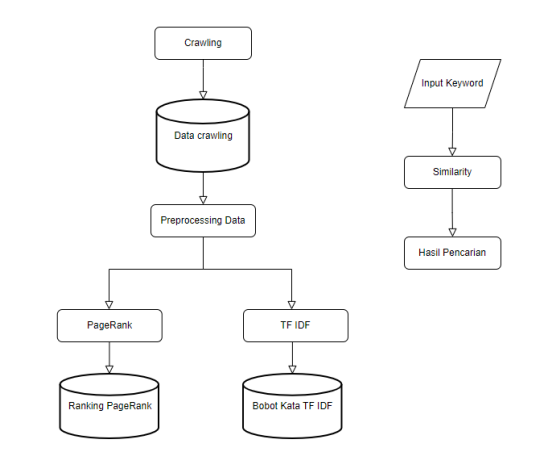
\includegraphics[width=\linewidth]{flowchart_lazuardy.png}
	\caption{\textit{Flowchart search engine}\cite{lazu}}
	\label{gambar:flowchart_lazu}
\end{figure}

Untuk \textit{web crawler} digunakan algoritma \textit{crawling} bernama \textit{breadth first search}. Pada Pada penerapannya, \textit{algoritma breadth first search} ini akan melakukan pencarian yang dimulai dari pemilihan \textit{node} awal kemudian dilanjutkan dengan pencarian bertahap level demi level. Algoritma ini merupakan bentuk paling sederhana dari algoritma \textit{crawling} \cite{lazu}. 

Pada saat tahap \textit{crawling}, digunakan pustaka \textit{beutifulsoup} python. Pustaka \textit{beautifulsoup} bertugas untuk mengolah setiap halaman yang algoritma \textit{crawling breadth first search} kunjungi untuk mendapatkan informasi yang akan disimpan dalam \textit{database} yang ada.

Preprocessing data dilakukan agar data yang digunakan bebas noise, memiliki ukuran yang lebih kecil, dan lebih terorganisir sehingga dapat diproses lebih lanjut \cite{lazu}.

Pada tahap selanjutnya setelah melewati tahap \textit{preprocessing data}, data dapat dilanjutkan ke dua tahap yaitu \textit{pagerank} dan \textit{tf-idf}. \textit{TF-IDF} adalah metode pemberian bobot pada hubungan antara kata (word) dan dokumen, metode ini adalah metode yang paling umum digunakan untuk menghitung bobot setiap kata dalam pencarian informasi \cite{lazu}. Pada tahapan \textit{pagerank} digunakan algoritma \textit{Pagerank} untuk menentukan peringkat halaman-halaman yang ada.


\subsection{\textit{Agile}}
Pengembangan perangkat lunak menggunakan agile merupakan salah satu metode pengembangan perangkat lunak yang ada. Kata "\textit{agile}" memiliki arti cepat, ringan dan bebas bergerak. Konsep pengembangan perangkat lunak menggunakan \textit{agile} ditemukan oleh Kent Beck dan 16 koleganya dengan menyatakan \textit{agile} adalah cara dalam membangun sebuah perangkat lunak dengan cara mengerjakannya dan membantu satu sama lain dalam membangunnya dalam satu waktu. Dalam pengembangan perangkat lunak menggunakan \textit{agile}, interaksi dan personil adalah hal yang penting dibandingkan proses dan alat kerja, Perangkat lunak yang bekerja lebih pentung dari dokumentasi yang lengkap, Kolaborasi antara klien lebih penting dari negosiasi kontrak dan responsif dalam perubahan adalah hal yang lebih penting dari mengikuti rencana yang telah dibuat. Spertim model lainnya, \textit{agile} memiliki kelebihan dan tidak cocok untuk semua tipe projek. \textit{Agile} membuat model proses yang toleran terhadap perubahan kebutuhan sehingga perubahan dapat dilakukan dengan cepat \cite{scrum}.

\subsection{\textit{Scrum}}

\textit{Scrum} adalah metodologi pengembangan dan manajemen yang dikembangkan oleh Jeff Sutherland pada tahun 1993, dengan tujuan mengikuti prinsip \textit{Agile}. Metode ini fokus pada strategi pengembangan perangkat lunak holistik, di mana tim pengembang bekerja sebagai satu unit untuk mencapai tujuan bersama.

Dalam pelaksanaannya, \textit{Scrum} terdiri dari tiga peran utama: \textit{Product Owner}, \textit{Scrum Master}, dan \textit{Team}. \textit{Product Owner} bertanggung jawab menentukan spesifikasi perangkat lunak dan membuat \textit{Product Backlog}. \textit{Team}, sebagai entitas pengembangan, bekerja untuk menyelesaikan tugas-tugas dalam \textit{Product Backlog}. \textit{Scrum Master} memperkenalkan dan mengimplementasikan metode \textit{Scrum} pada tim.

Proses pengerjaan projek dengan \textit{Scrum} dimulai dengan penggambaran sistem yang akan dibuat, kemudian \textit{Product Owner} menggambarkan proses bisnis ke dalam Product Backlog. \textit{Sprint}, sebagai bagian dari \textit{Scrum}, adalah tujuan yang ingin dicapai dalam iterasi selanjutnya. Setiap sprint dimulai dengan \textit{Sprint Planning Meeting}, diikuti oleh pertemuan harian \textit{Daily Scrum Meeting} di mana setiap anggota tim berdiskusi tentang progres dan tugas selanjutnya. \textit{Sprint} diakhiri dengan pertemuan untuk mendemonstrasikan hasil pekerjaan. \textit{Scrum} dirancang untuk meningkatkan fleksibilitas dan responsivitas dalam pengembangan perangkat lunak \cite{scrum}.

%------------------------------------------------

\section{Pengembangan}

\subsection{Pengembangan Dengan \textit{Scrum}}
Agar penelitian ini menjadi lebih terstruktur dan mudah, maka penelitian ini
akan menggunakan metode \textit{scrum} sebagai metode pengembangan sistemnya.
Komponen-komponen \textit{scrum} terdiri dari \textit{product backlog}, \textit{sprint backlog}, \textit{daily scrum} dan \textit{sprint} lalu dilanjutkan dengan pengujian sistem yang sudah dibuat.

\begin{figure}[H]
	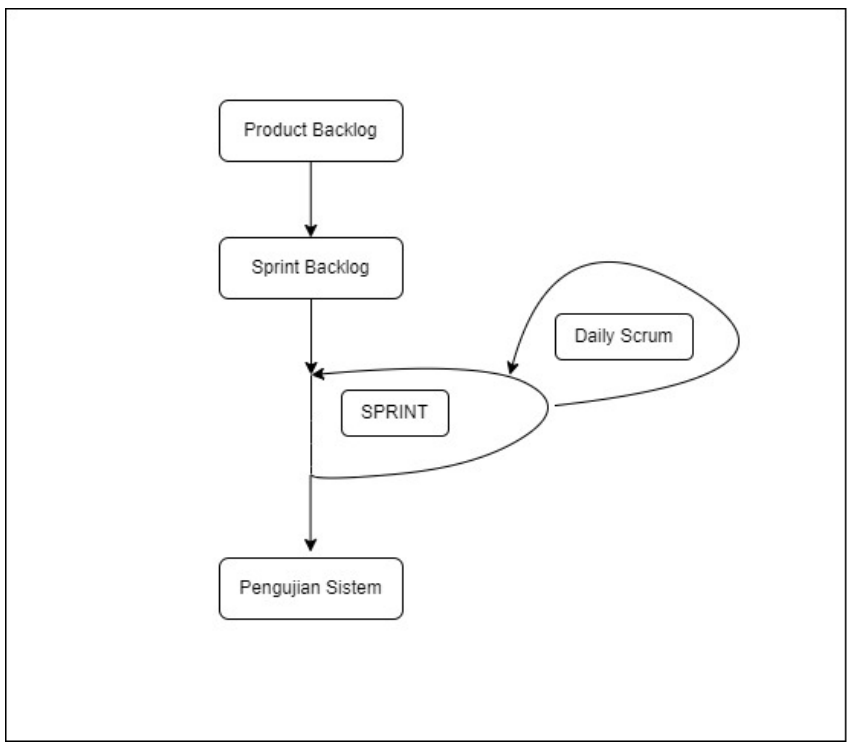
\includegraphics[width=\linewidth]{desain-penelitian.png}
	\caption{Tahapan penelitian dengan menggunakan metode \textit{scrum}}
\end{figure}

\subsubsection{\textit{Product Backlog}}
\textit{Product backlog} merupakan kumpulan tugas yang akan dilaksanakan. \textit{Product backlog} seperti ditunjukan oleh tabel \ref{table:productbacklog} terdiri dari 3 komponen yaitu \textit{story}, \textit{sprint} dan \textit{status}. \textit{Story} ialah sebuah pekerjaan besar yang dapat dibagi bagi lebih kecil lagi menjadi tugas tugas kecil. \textit{Sprint} menandakan sprint berapa story tersebut akan diselesaikan. \textit{Status} memberitahu apakah sprint tersebut sudah terlaksanakan atau belum.

\begin{table}[H]
	\centering
	\caption{\textit{Product Backlog}}
	\label{table:productbacklog}
	\begin{tabular}{@{} |p{0.25cm}|p{3cm}| p{1cm} |p{1cm}|@{}}
		\hline
		\textbf{No.} & \textbf{\textit{Story}} & \textbf{\textit{Sprint}} & \textbf{\textit{Status}} \\
		\hline
		1 & Fitur pencarian pengguna & 1, 2, 8 & Selesai \\
		\hline
		2 & Fitur \textit{page ranking} & 4, 5 & Selesai\\
		\hline
		3 & Fitur \textit{staff} & 5, 8 & Selesai\\
		\hline
		4 & Fitur \textit{document ranking} & 5, 7  & Selesai\\
		\hline
		5 & Fitur \textit{crawling} & 3, 6 & Selesai\\
		\hline
		6 & Struktur projek & 2 & Selesai\\
		\hline
		7 & \textit{multi-threaded service} & 10  & Selesai\\
		\hline
		8 & \textit{Service deployment} & 11  & Selesai\\
		\hline
		9 & Background task dengan \textit{Celery} & 12  & Selesai\\
		\hline
		10 & Pengujian penggunaan memori & 13  & Selesai\\
		\hline
	\end{tabular}
\end{table}

\subsubsection{\textit{Sprint Backlog}}
\textit{Sprint backlog} merupakan daftar tugas tugas kecil yang perlu dilaksanakan pada suatu \textit{sprint}.

\subsubsection{\textit{Sprint}}
\textit{Sprint} merupakan masa dimana pengerjaan tugas tugas yang telah direncanakan pada suatu \textit{sprint} dilakukan. Lama durasi setiap \textit{sprint} ditentukan oleh \textit{scrum} \textit{master} yang telah disepakati bersama

\subsubsection{\textit{Daily Scrum}}
\textit{Daily scrum} merupakan pertemuan dengan \textit{scrum master} untuk membahas tugas apa yang telah dicapai hari kemarin dan tugas apa yang ingin dicapai hari ini yang dilaksanakan setiap hari.

\subsection{Analisis Kebutuhan}
Analisis kebutuhan dilakukan guna mengumpulkan informasi mengenai kebutuhan fitur aplikasi dan prioritas fitur aplikasi yang akan dibuat. Dari analisis kebutuhan yang dilakukan dihasilkan sebuah \textit{usecase diagram} yang didefinisikan sebagai berikut.


\begin{figure}[H]
	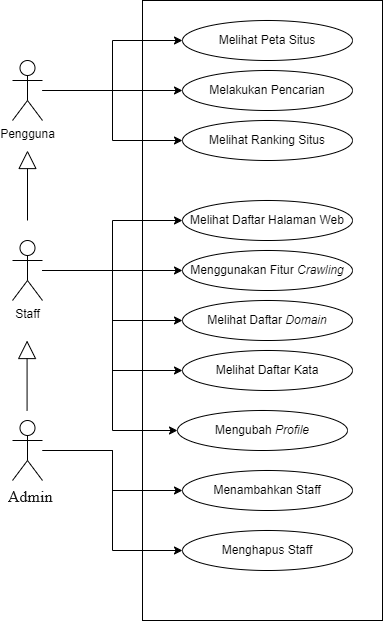
\includegraphics[width=\linewidth]{usecase.png}
	\caption{\textit{Use case diagram}}
\end{figure}



\section{Hasil dan Pembahasan}


\subsection{Implementasi \textit{User Interface}}

Pada implementasi \textit{user interface}, digunakan bahasa pemrograman \textit{javascript}. Adapun hasil implementasi \textit{user interface} sebagai berikut

\begin{figure}[H]
	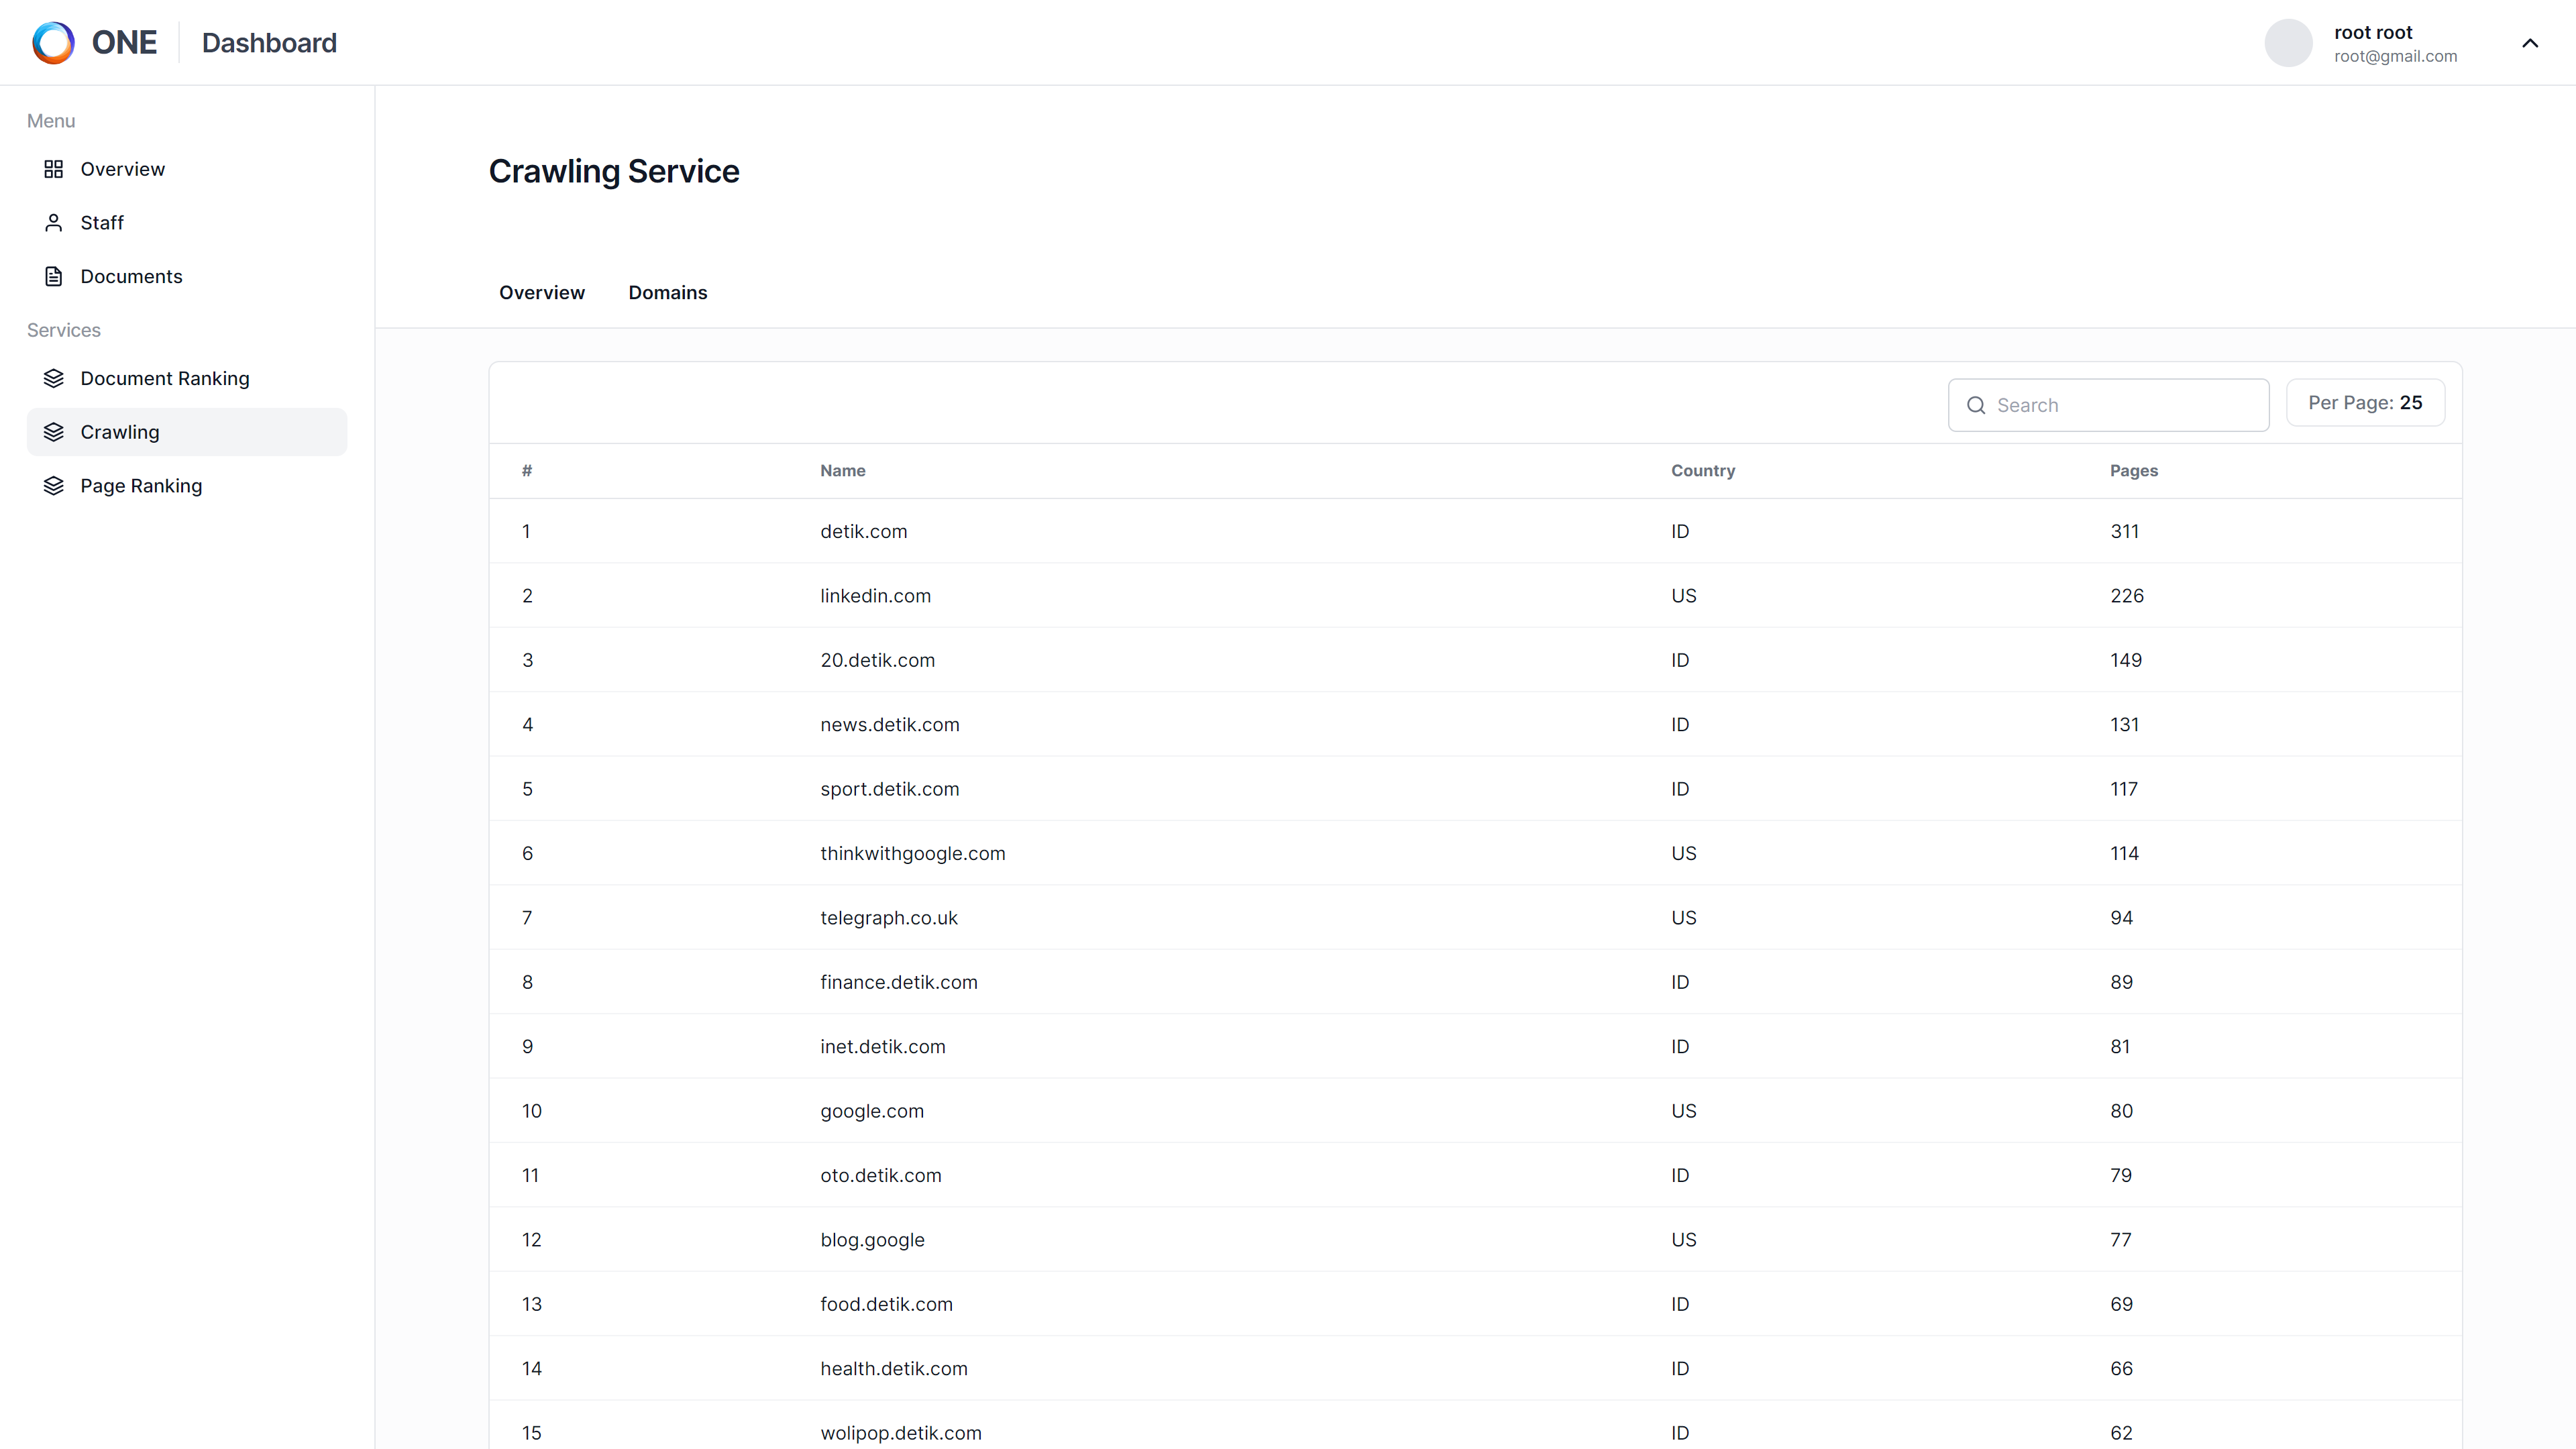
\includegraphics[width=\linewidth]{view_crawling_domain_list.png}
	\caption{Halaman Daftar Domain}
	\label{gambar:halaman_daftar_domain}
\end{figure}
\begin{figure}[H]
	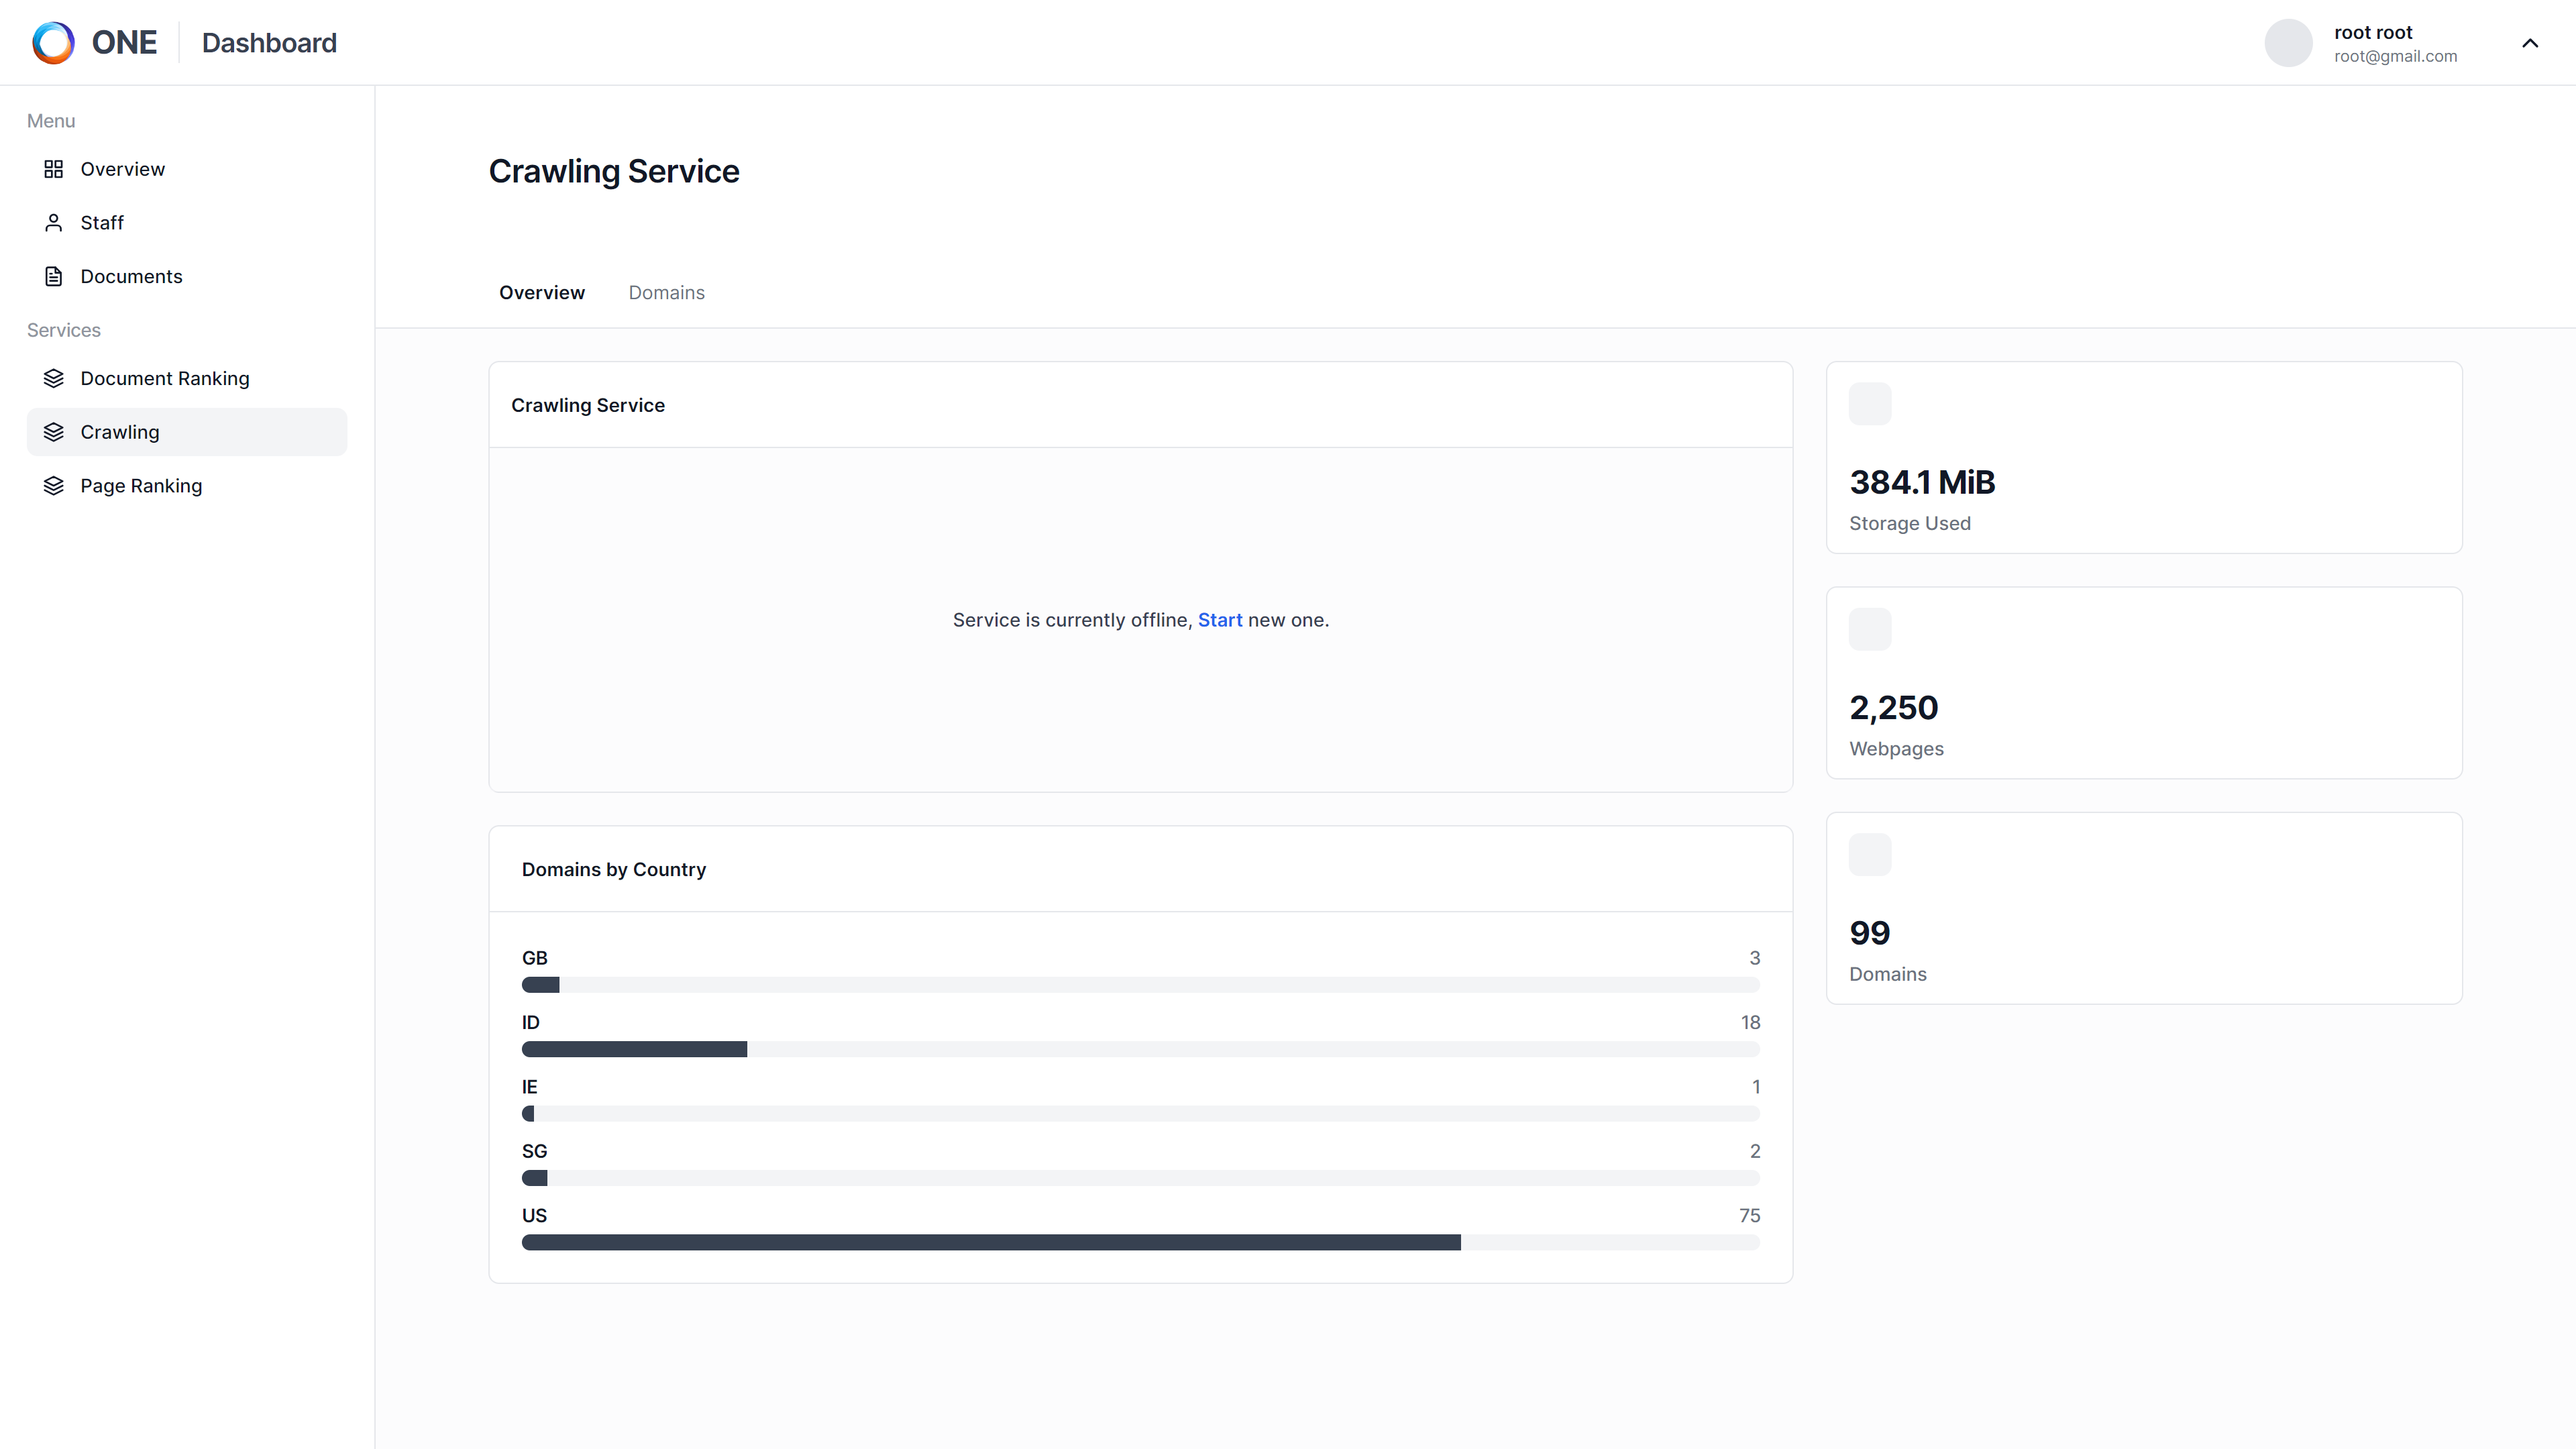
\includegraphics[width=\linewidth]{view_dashboard_services_crawling_overview.png}
	\caption{Halaman \textit{Service Crawling}}
	\label{gambar:halaman_dashboard_service_crawling}
\end{figure}
\begin{figure}[H]
	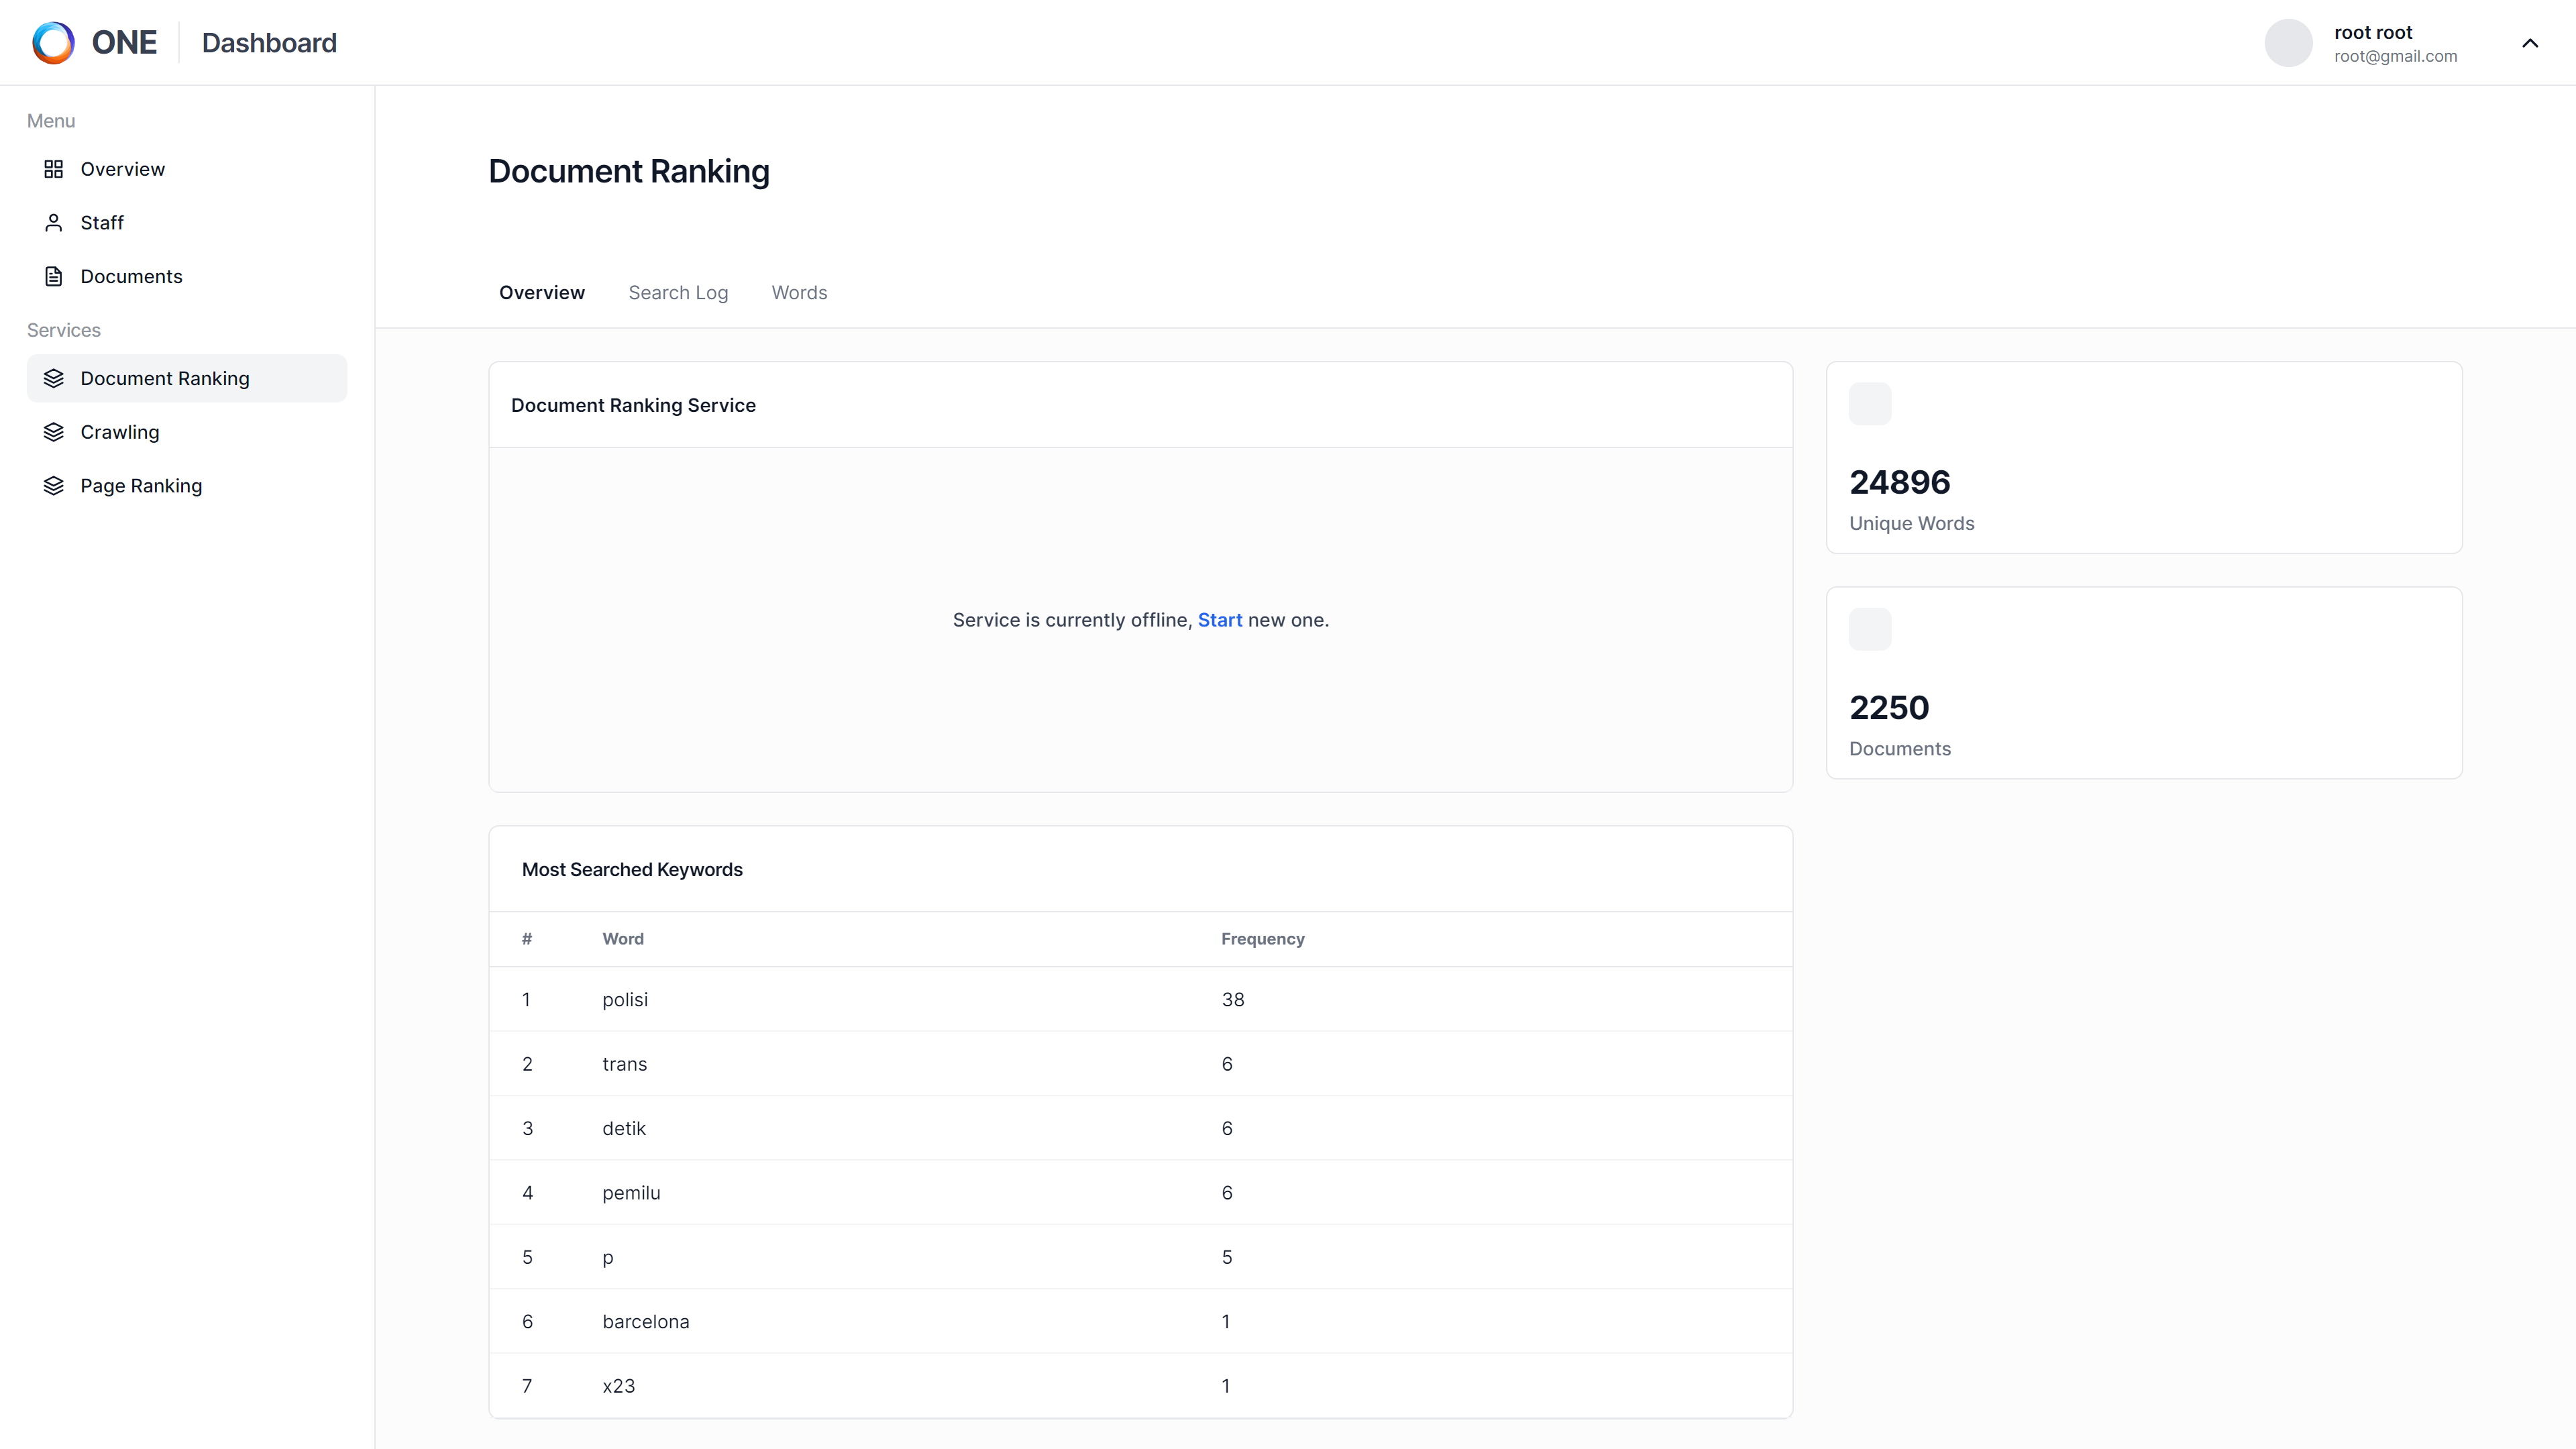
\includegraphics[width=\linewidth]{view_document_ranking_overview.png}
	\caption{Halaman \textit{Document Ranking}}
	\label{gambar:halaman_document_ranking_overview}
\end{figure}
\begin{figure}[H]
	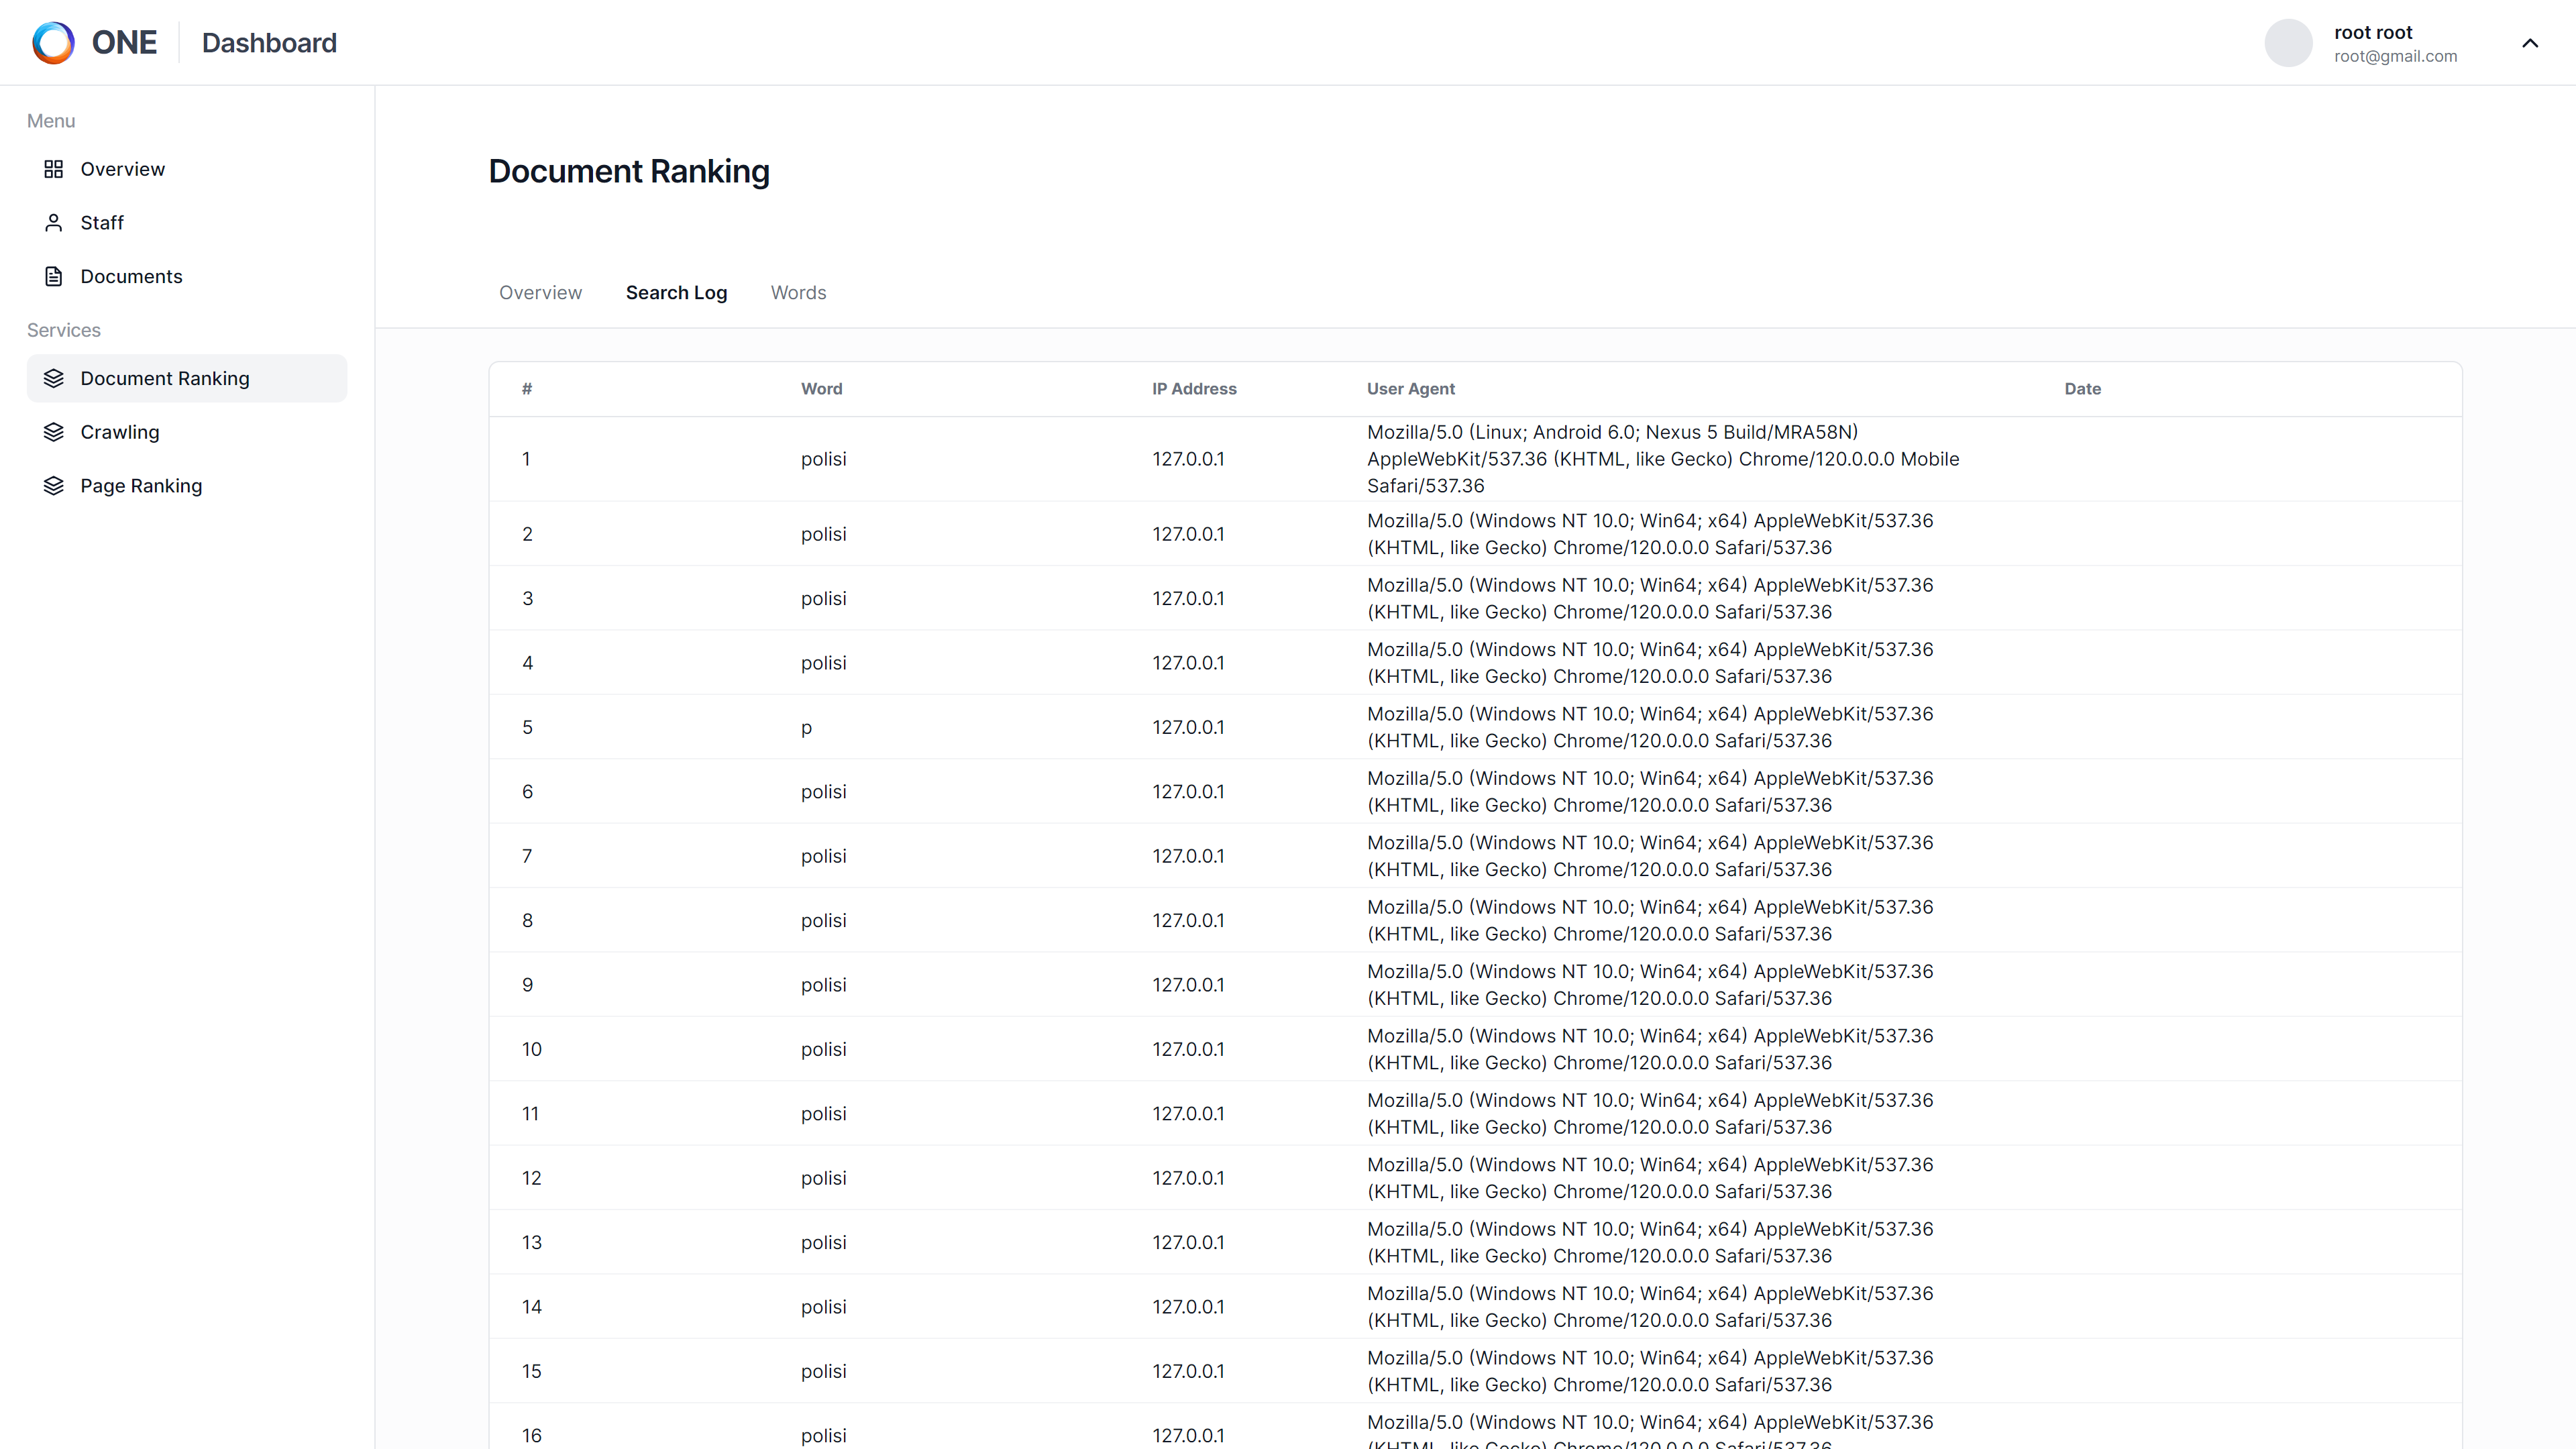
\includegraphics[width=\linewidth]{view_document_ranking_search_logs.png}
	\caption{Halaman \textit{search log}}
	\label{gambar:halaman_search_log}
\end{figure}
\begin{figure}[H]
	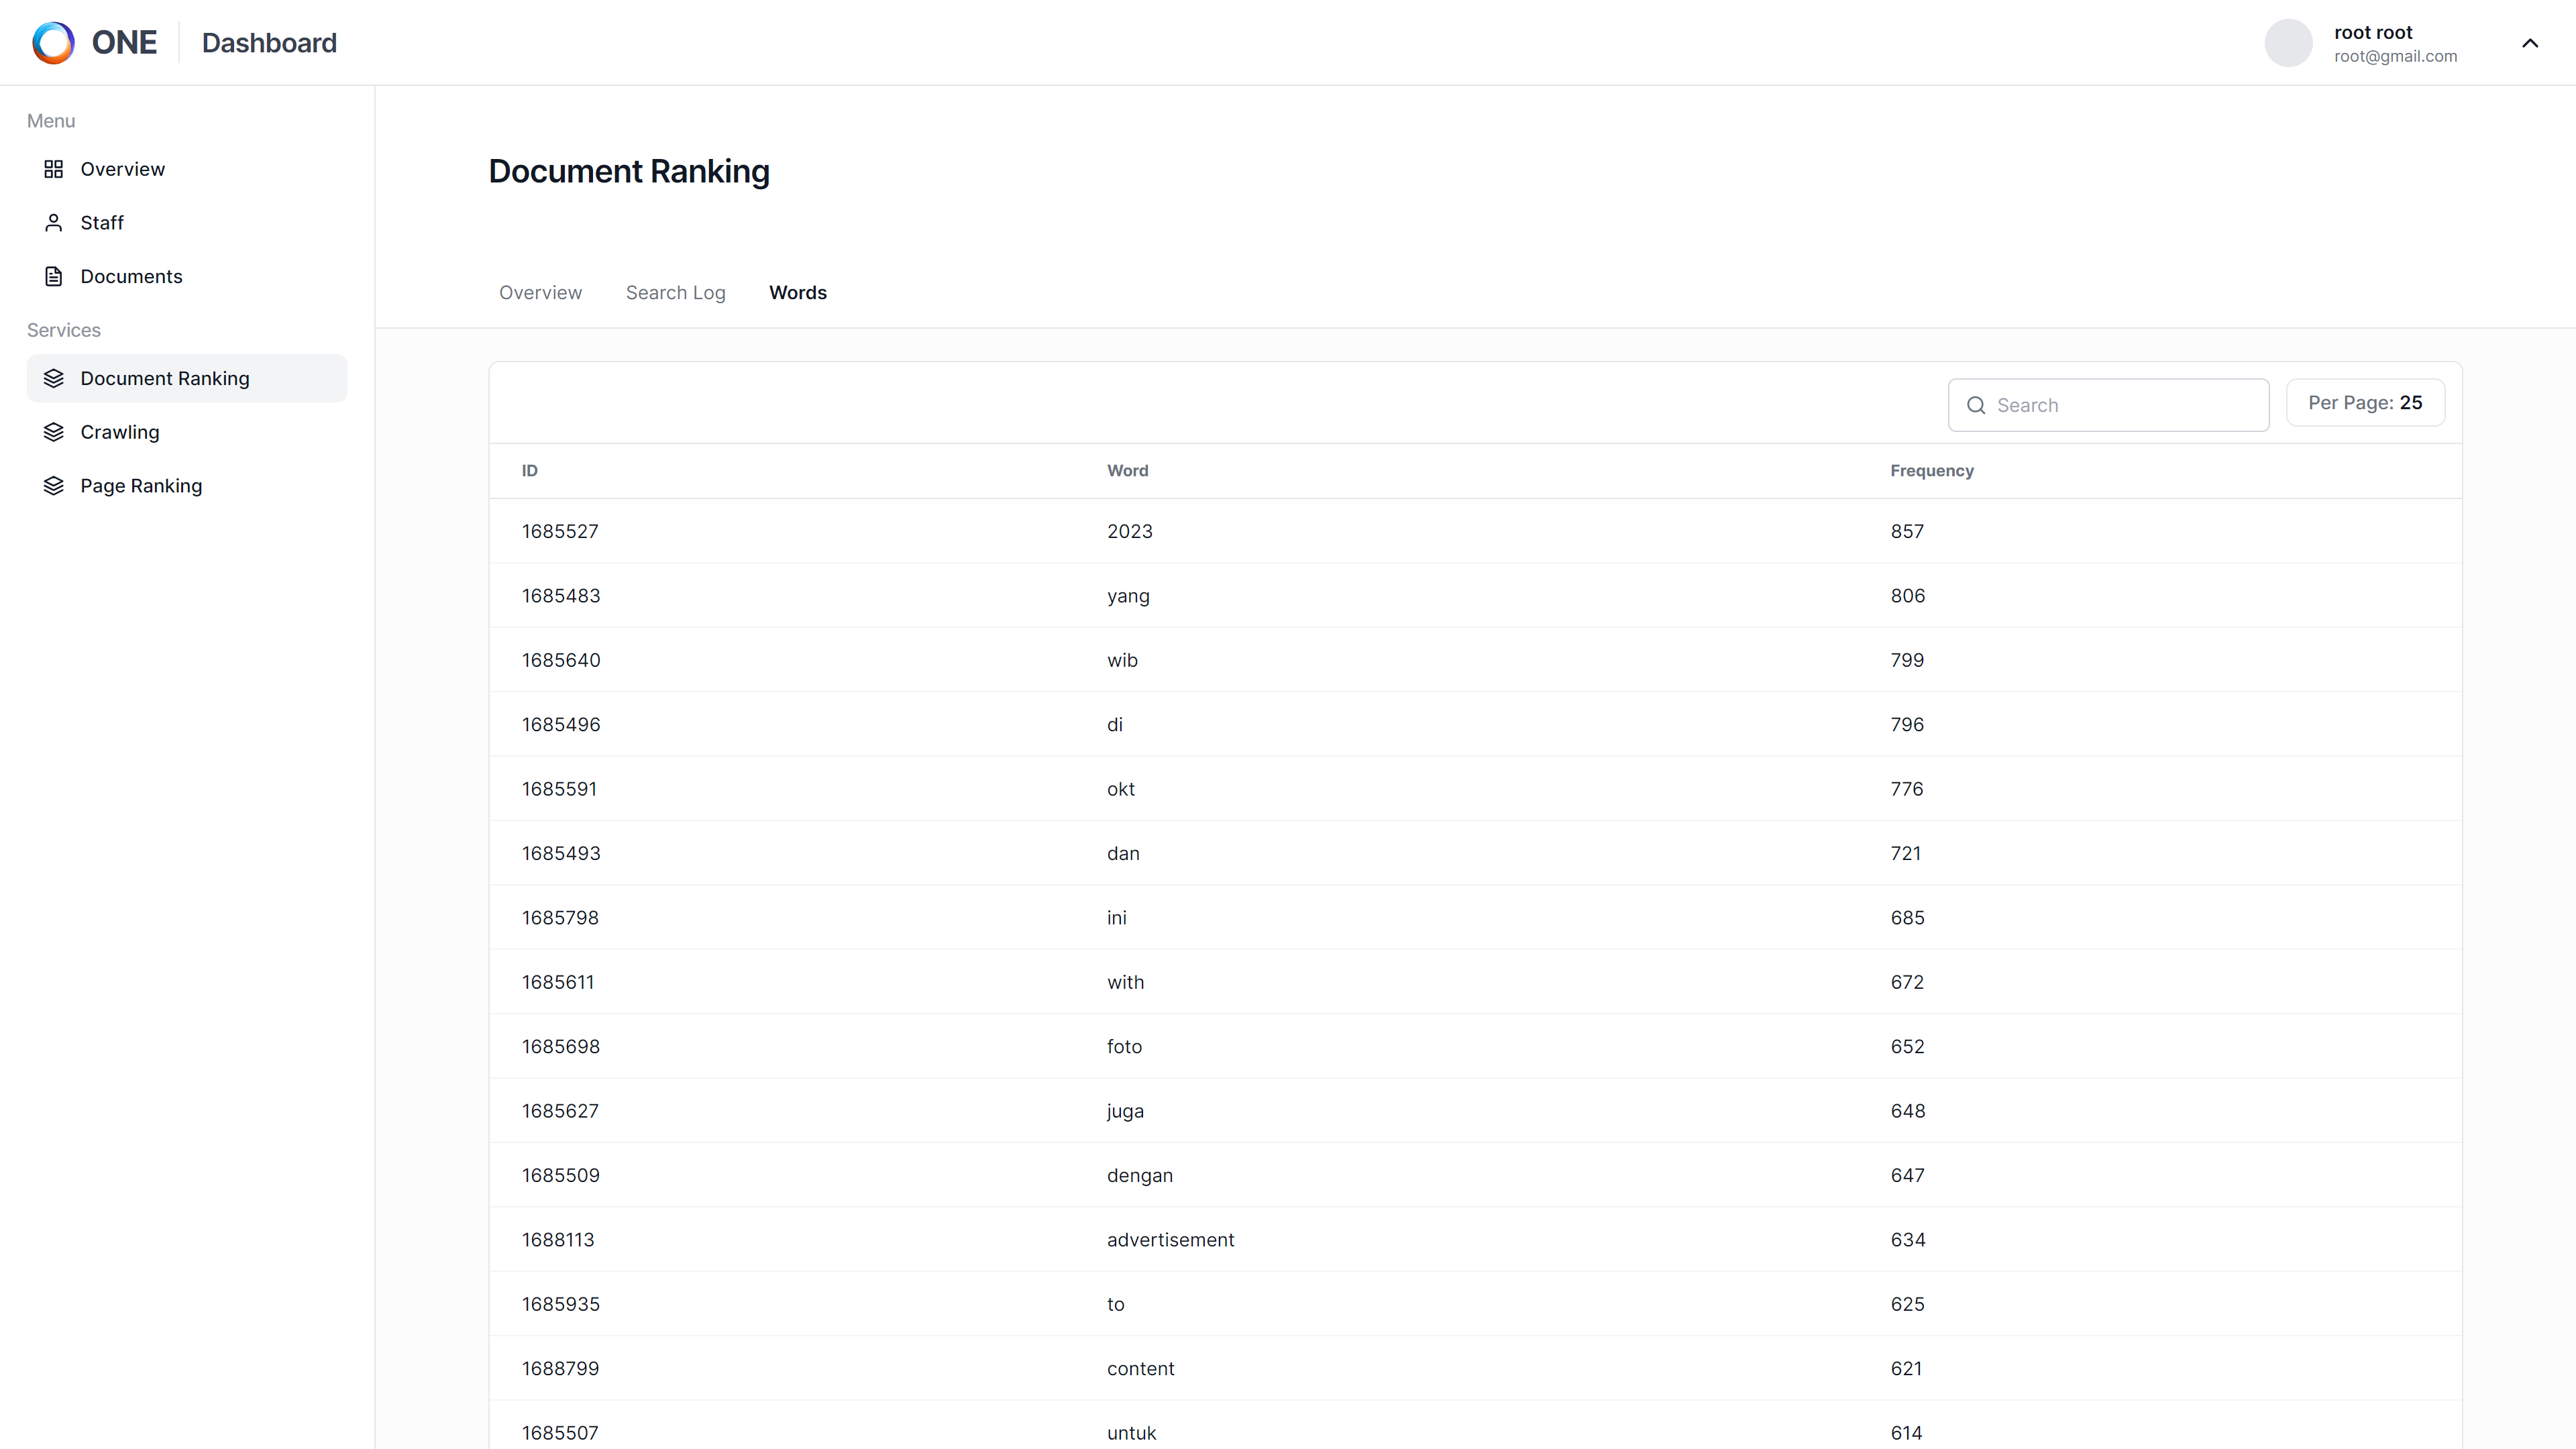
\includegraphics[width=\linewidth]{view_document_ranking_words.png}
	\caption{Halaman \textit{words}}
	\label{gambar:halaman_words}
\end{figure}
\begin{figure}[H]
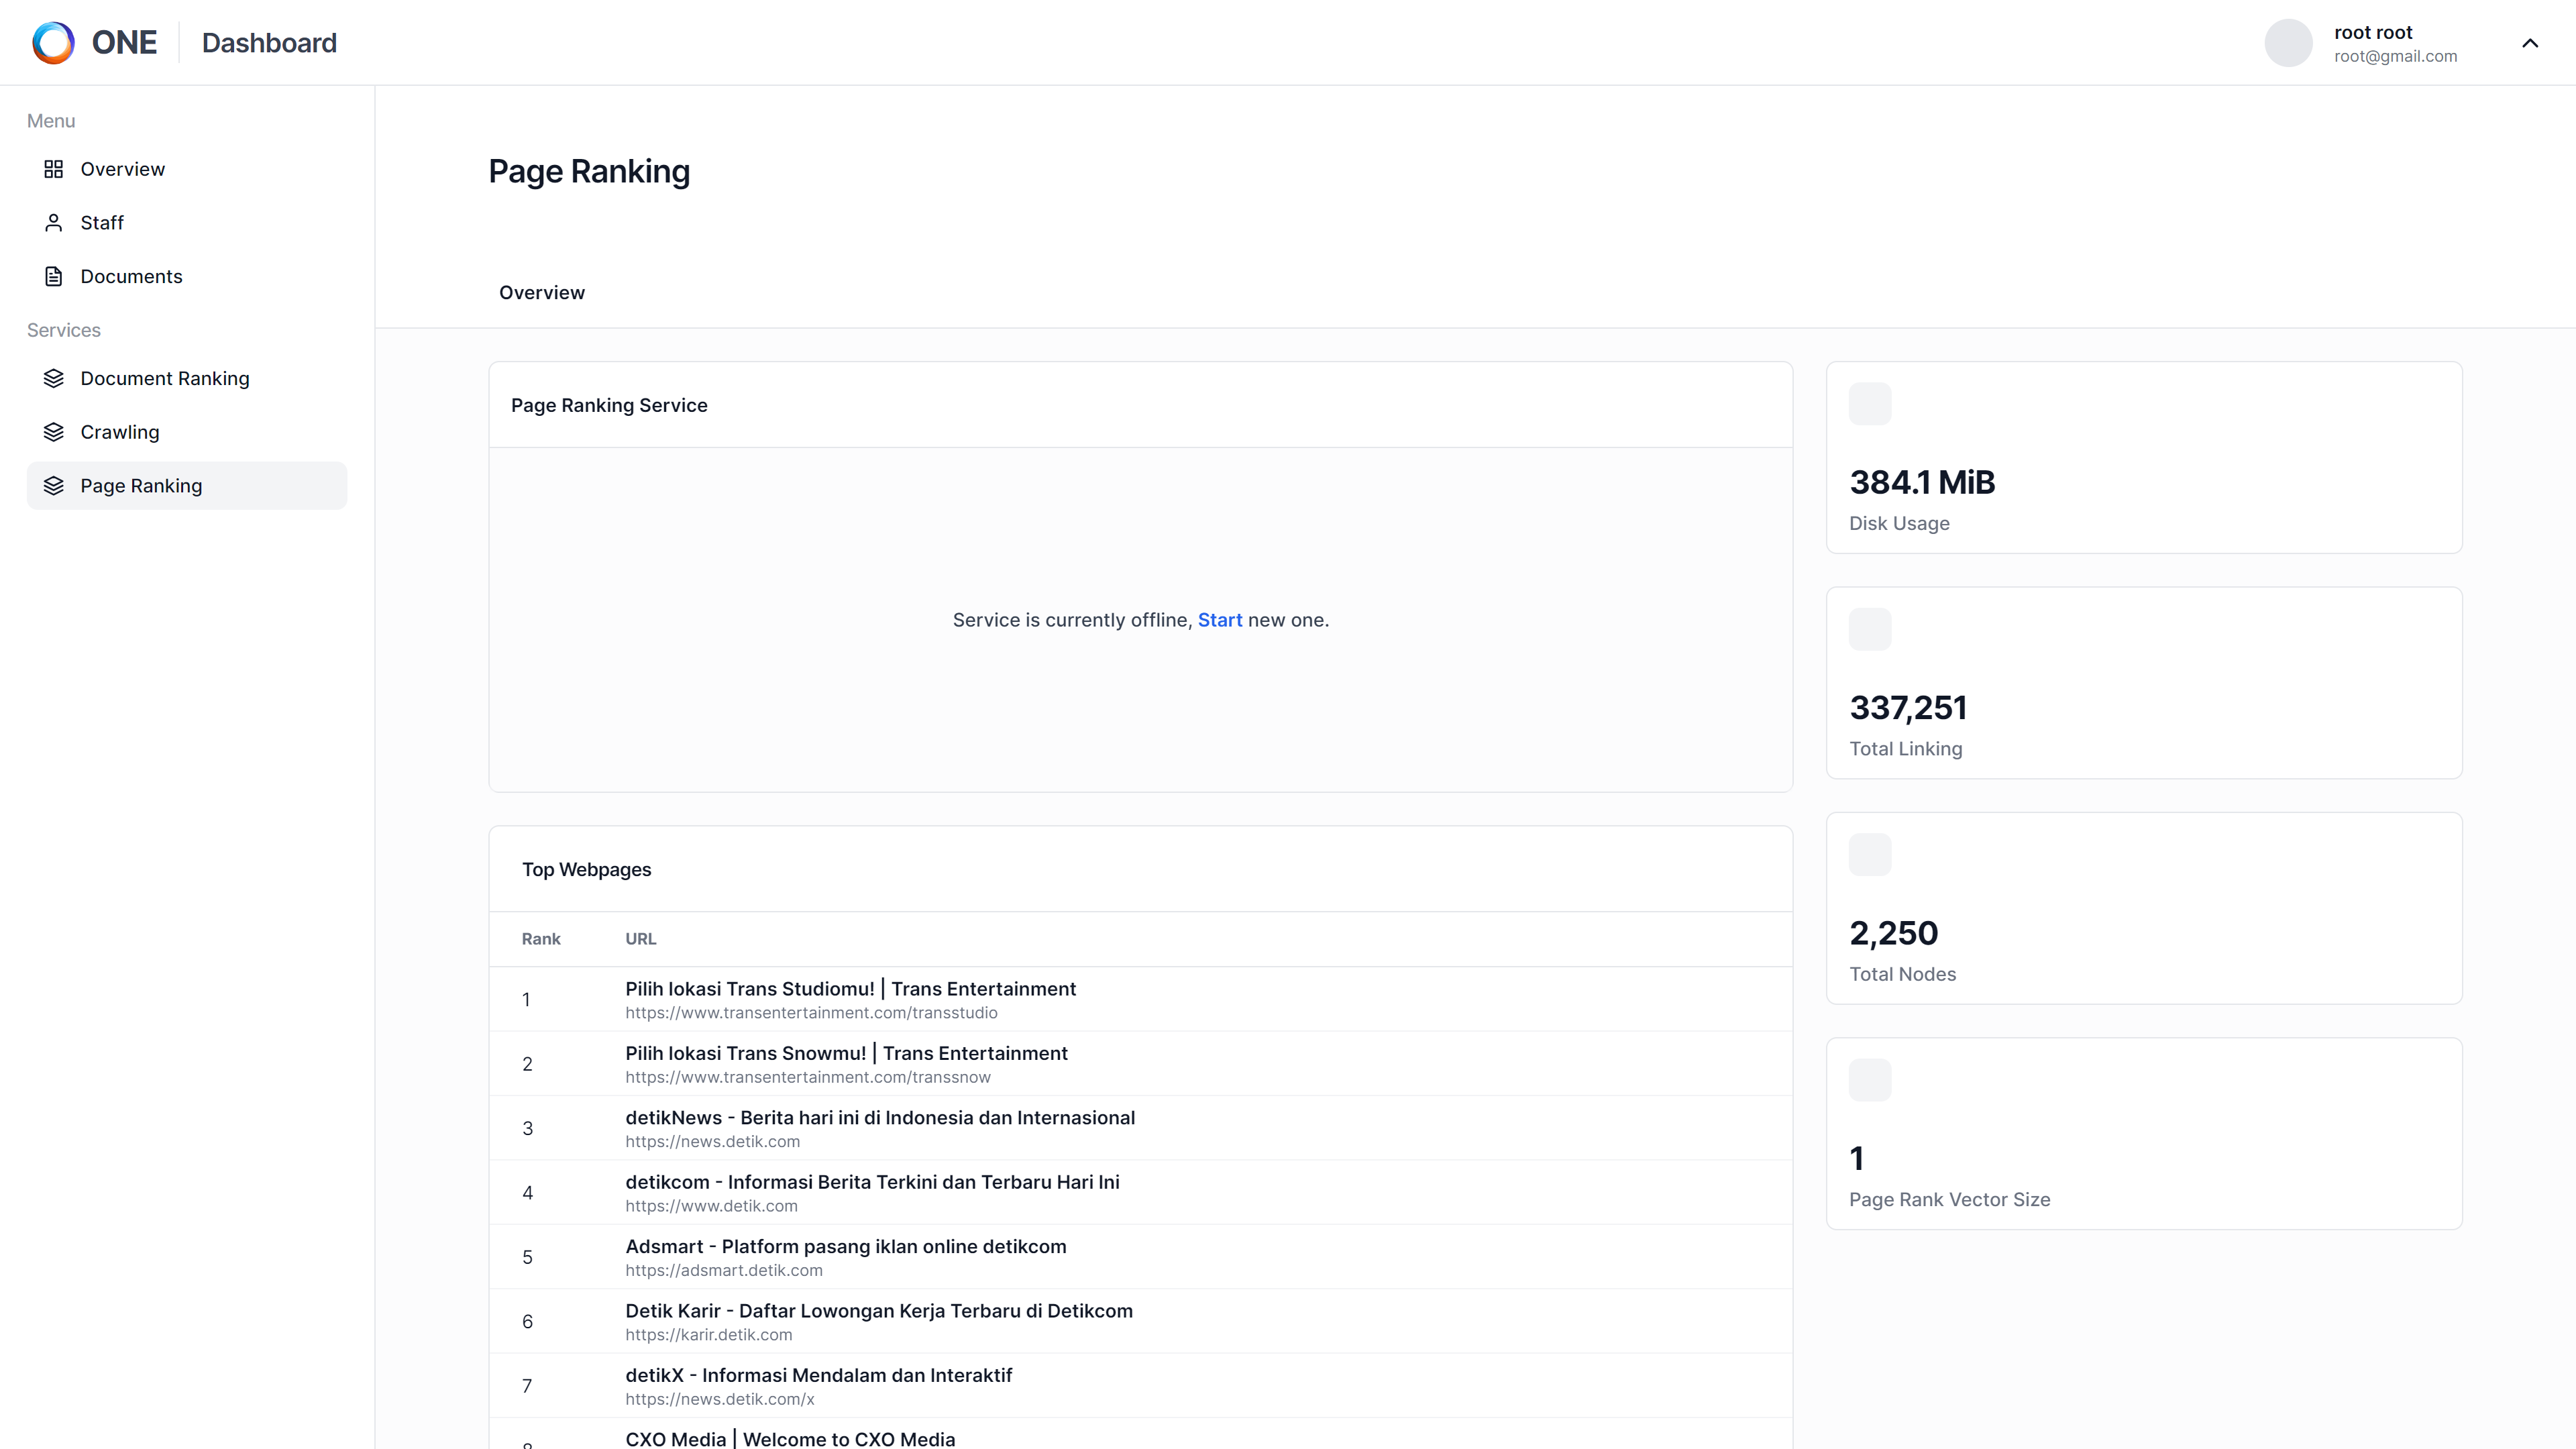
\includegraphics[width=\linewidth]{view_page_ranking_overview.png}
\caption{Halaman \textit{page ranking}}
\label{gambar:halaman_page_ranking}
\end{figure}
\begin{figure}[H]
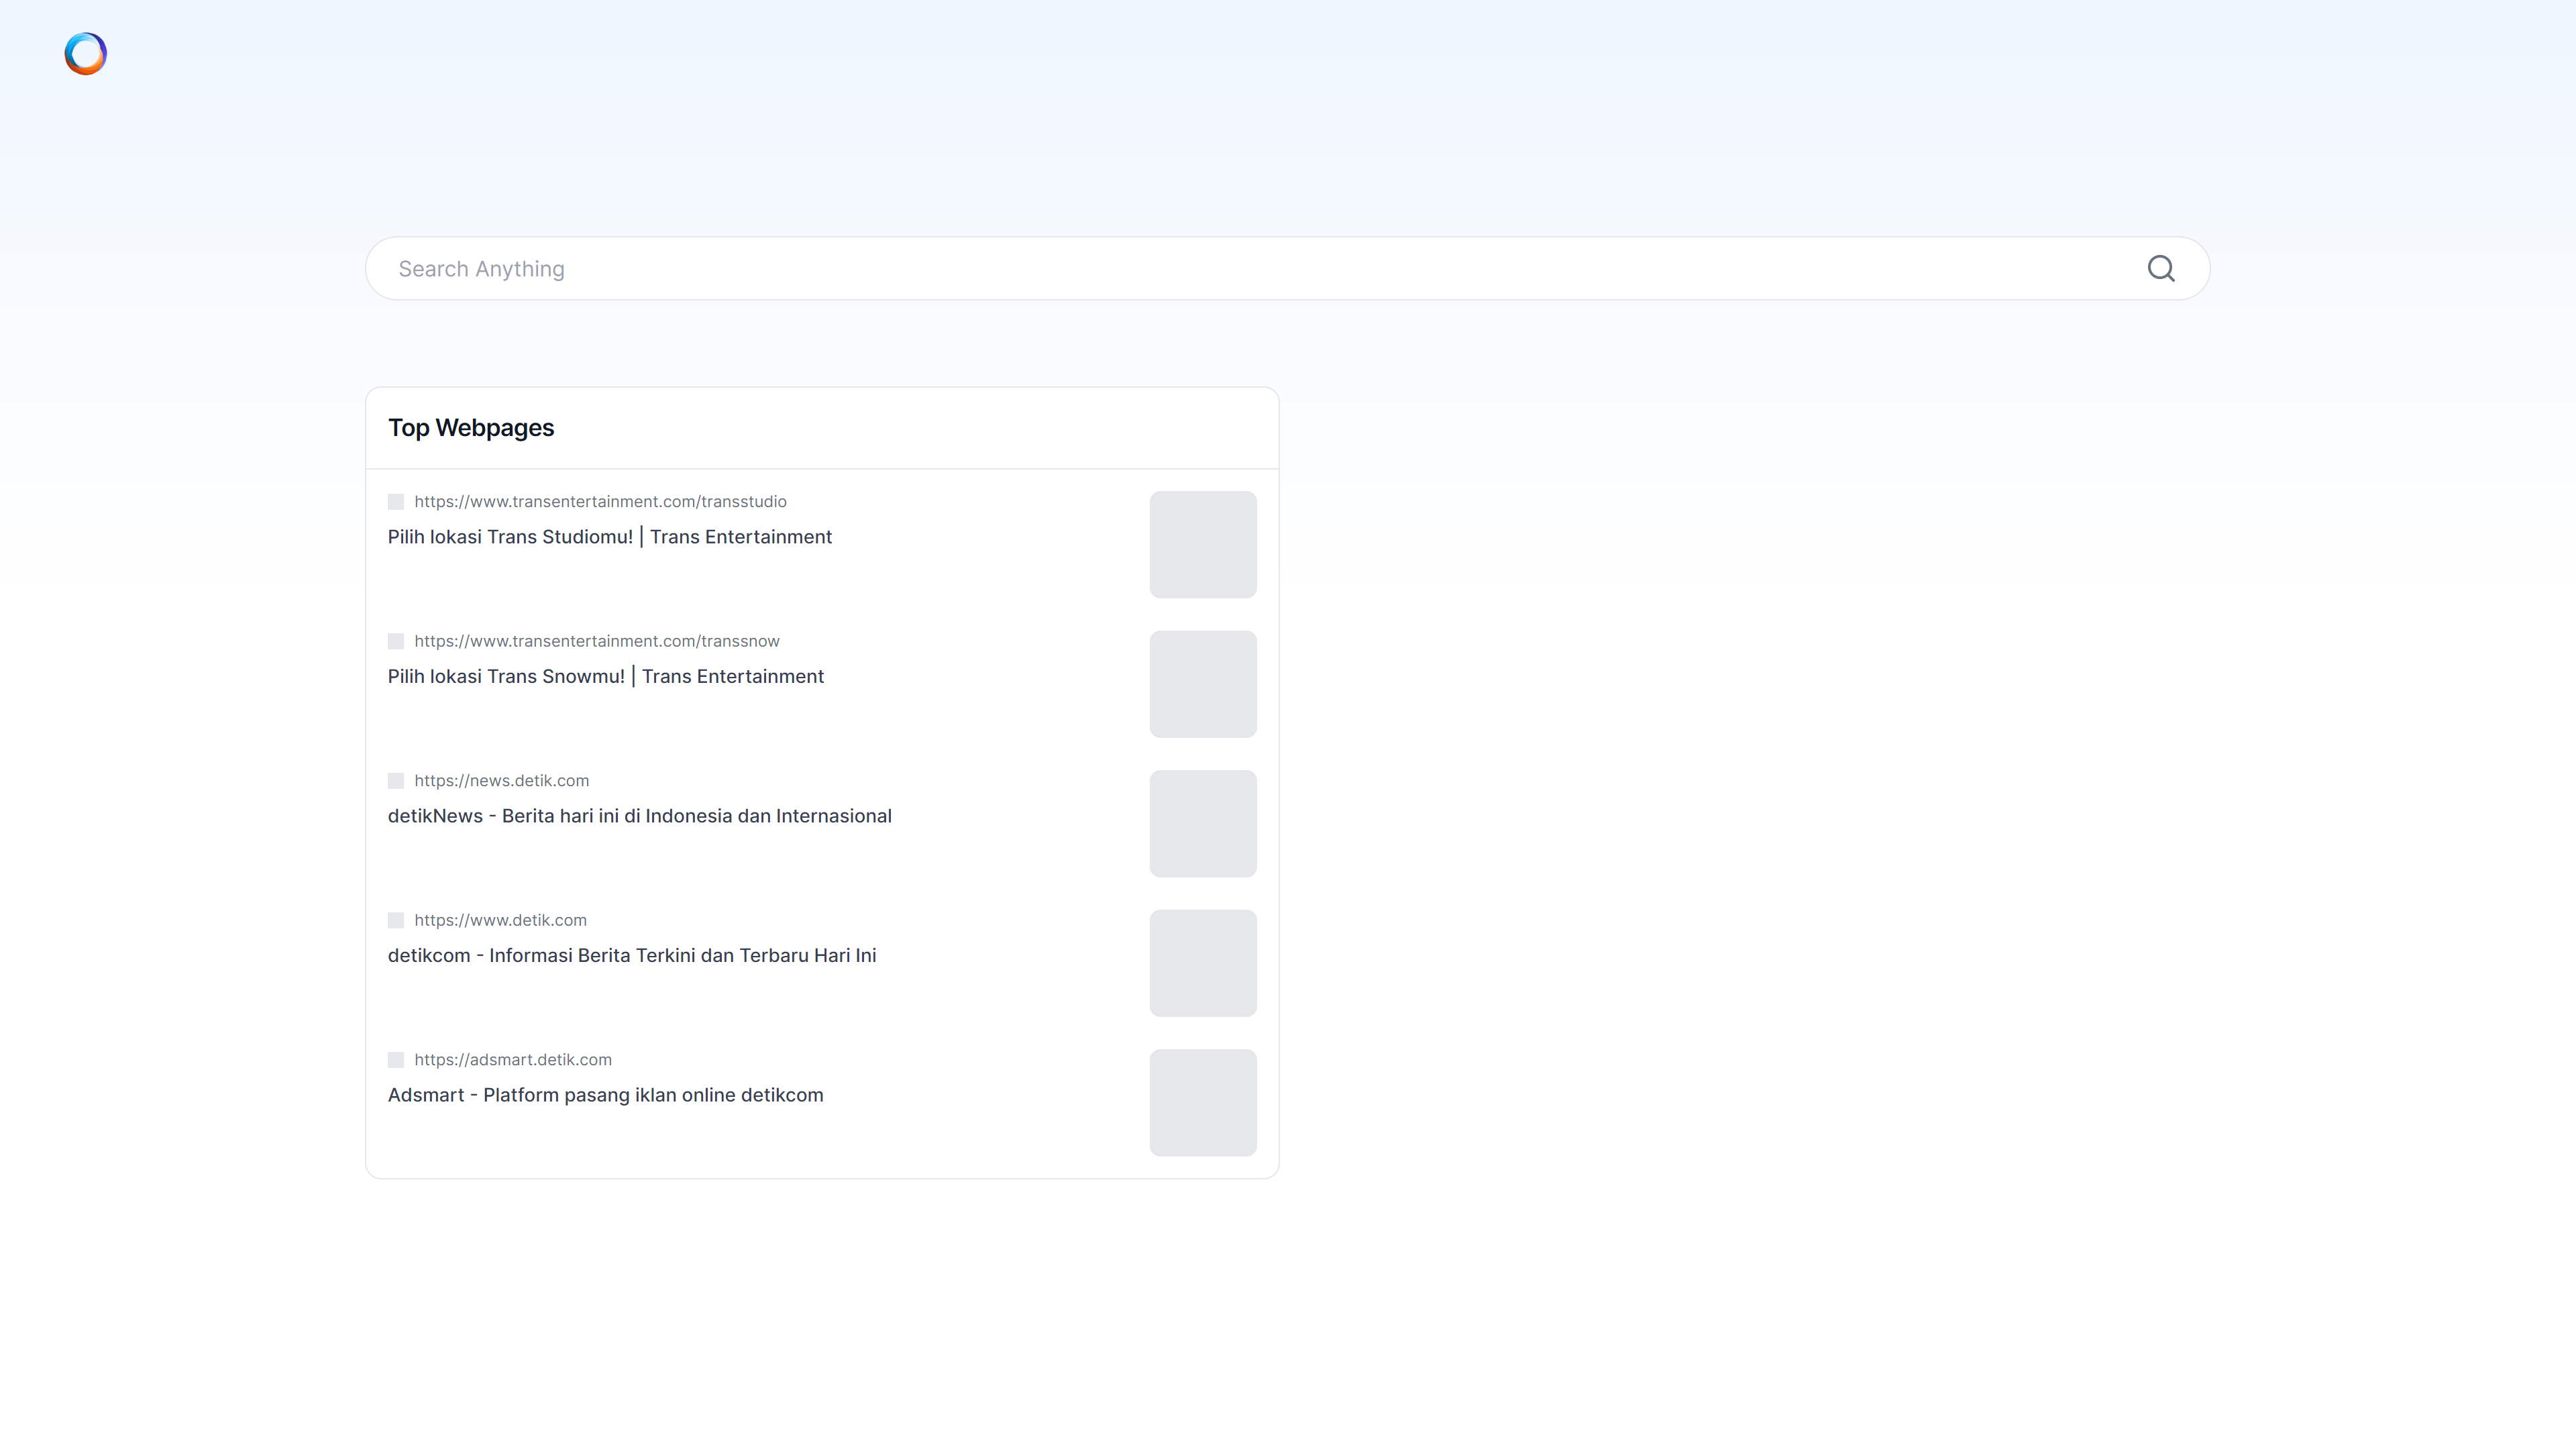
\includegraphics[width=\linewidth]{view_search_engine_home.png}
\caption{Halaman pencarian}
\label{gambar:halaman_search_engine}
\end{figure}
\begin{figure}[H]
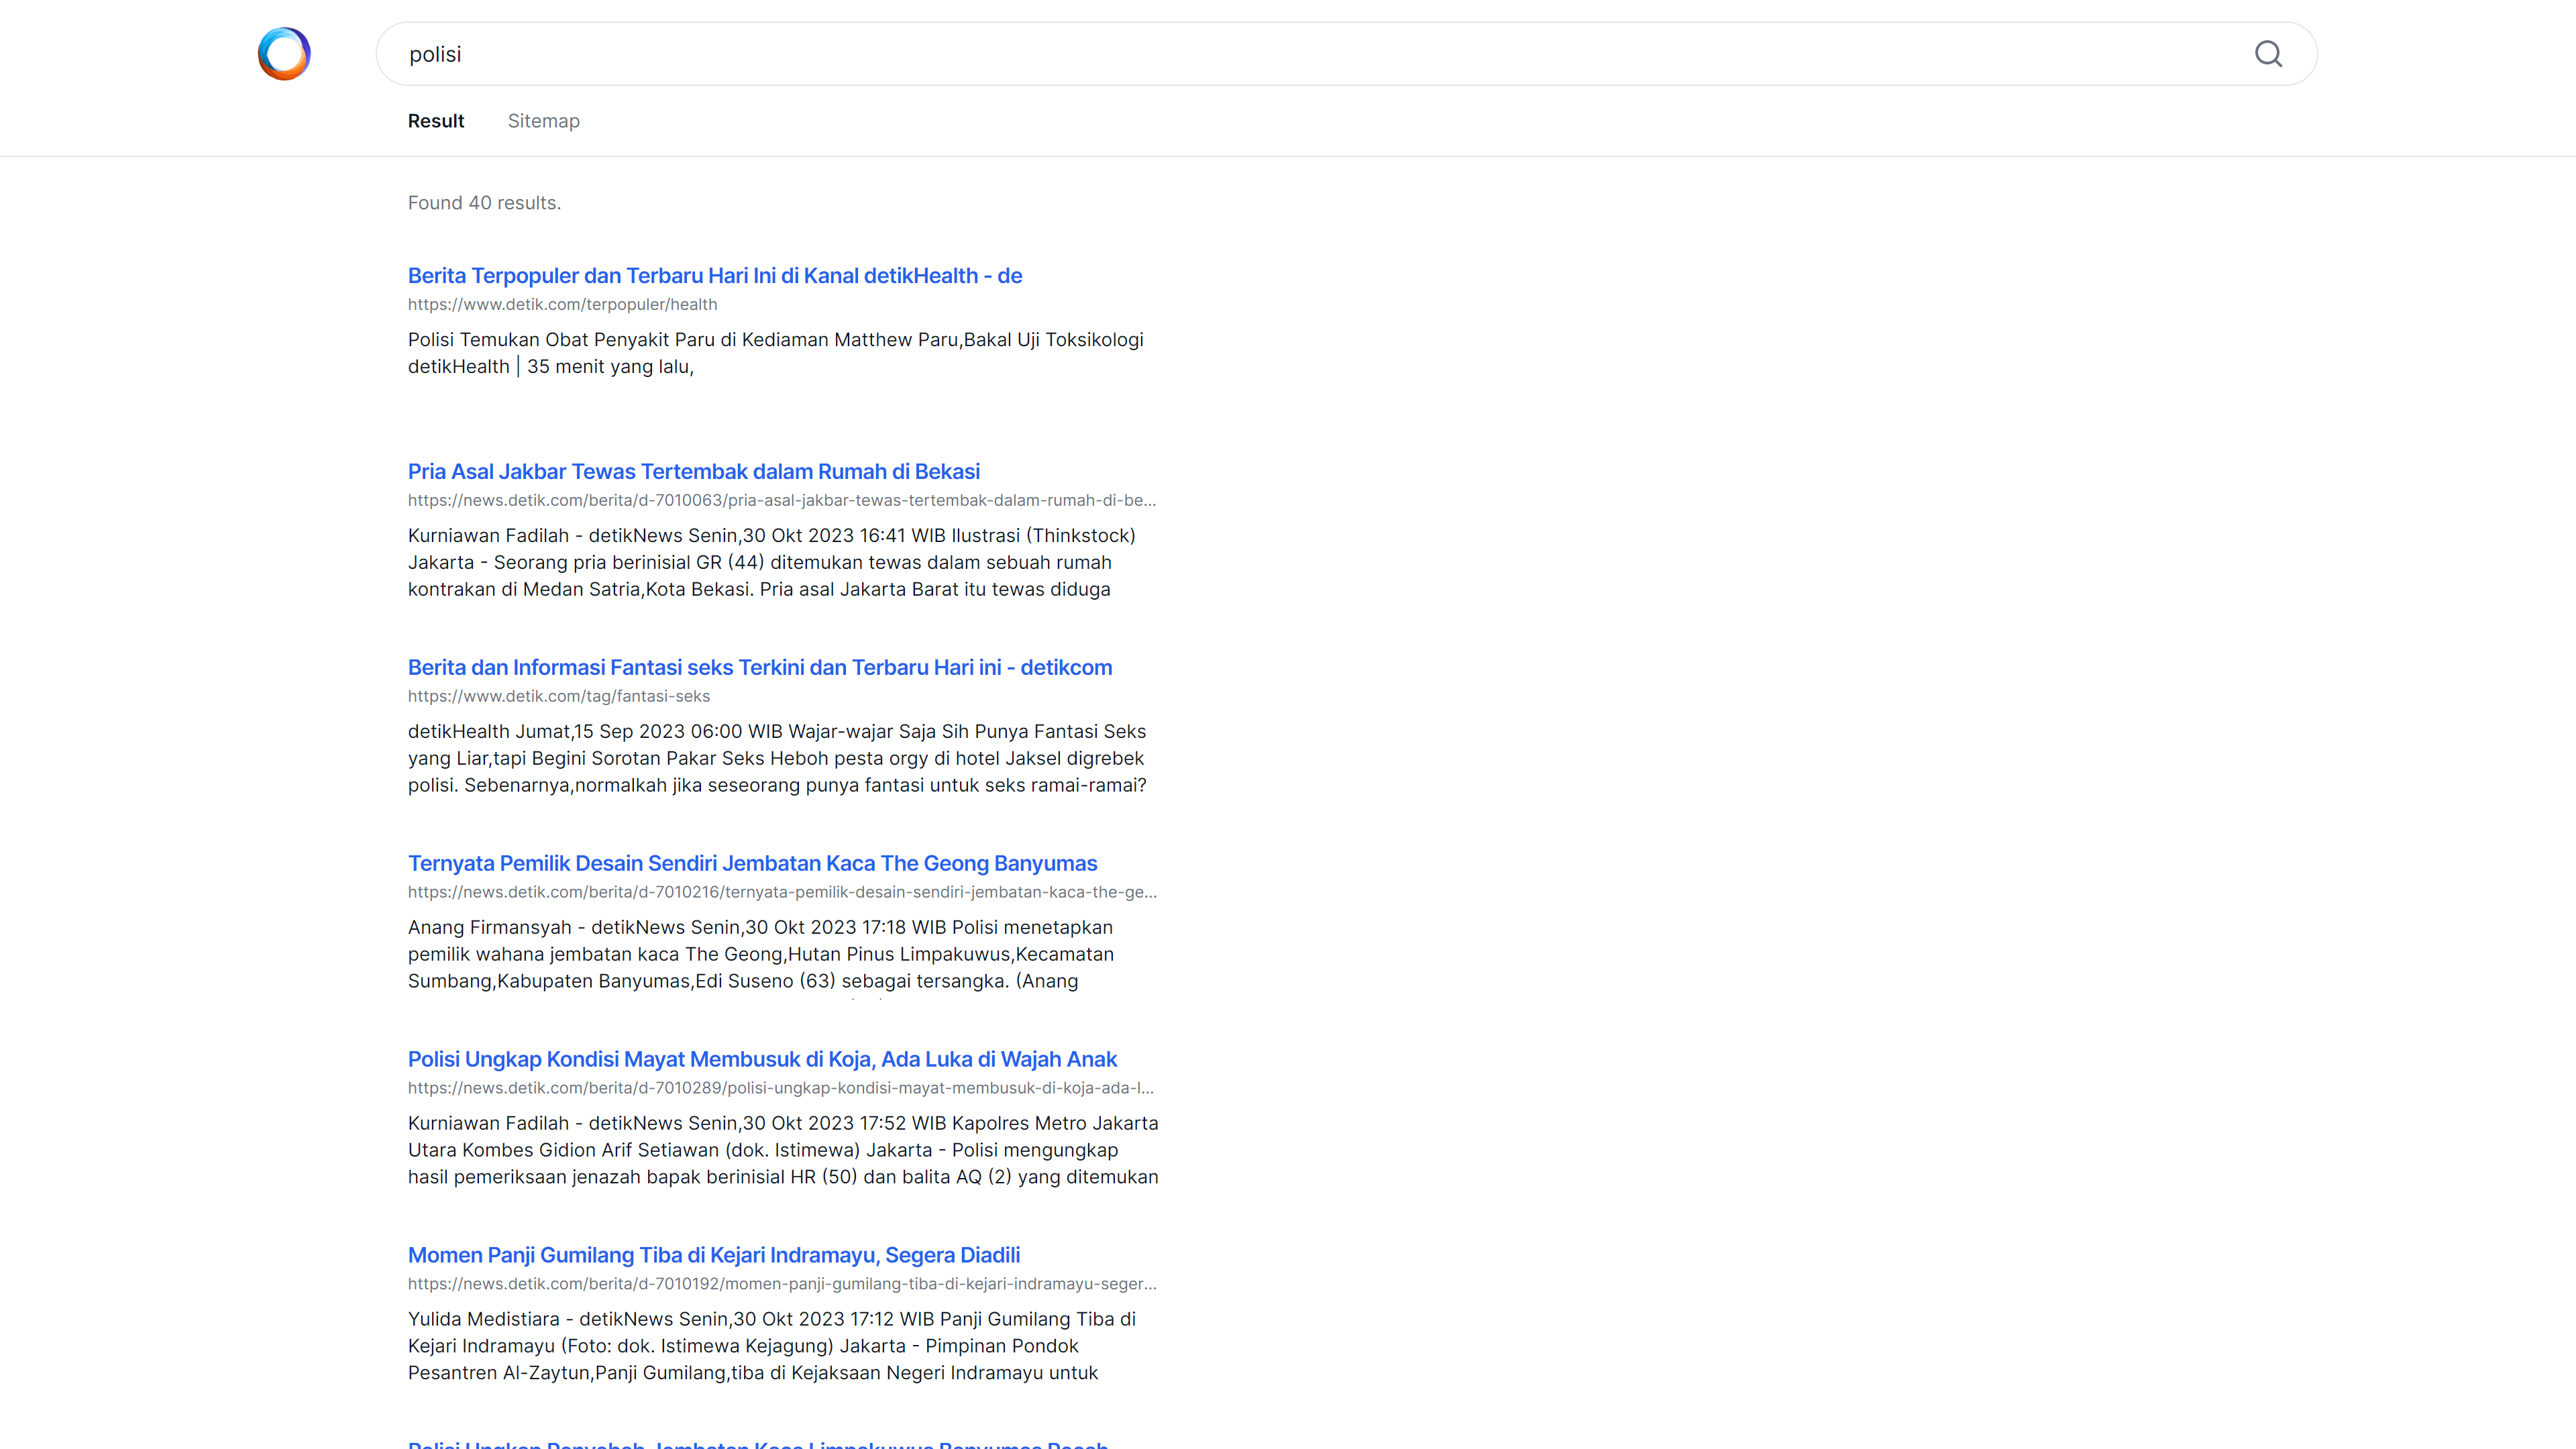
\includegraphics[width=\linewidth]{view_search_engine_result.png}
\caption{Halaman hasil pencarian}
\label{gambar:halaman_hasil_pencarian}
\end{figure}

\begin{figure}[H]
	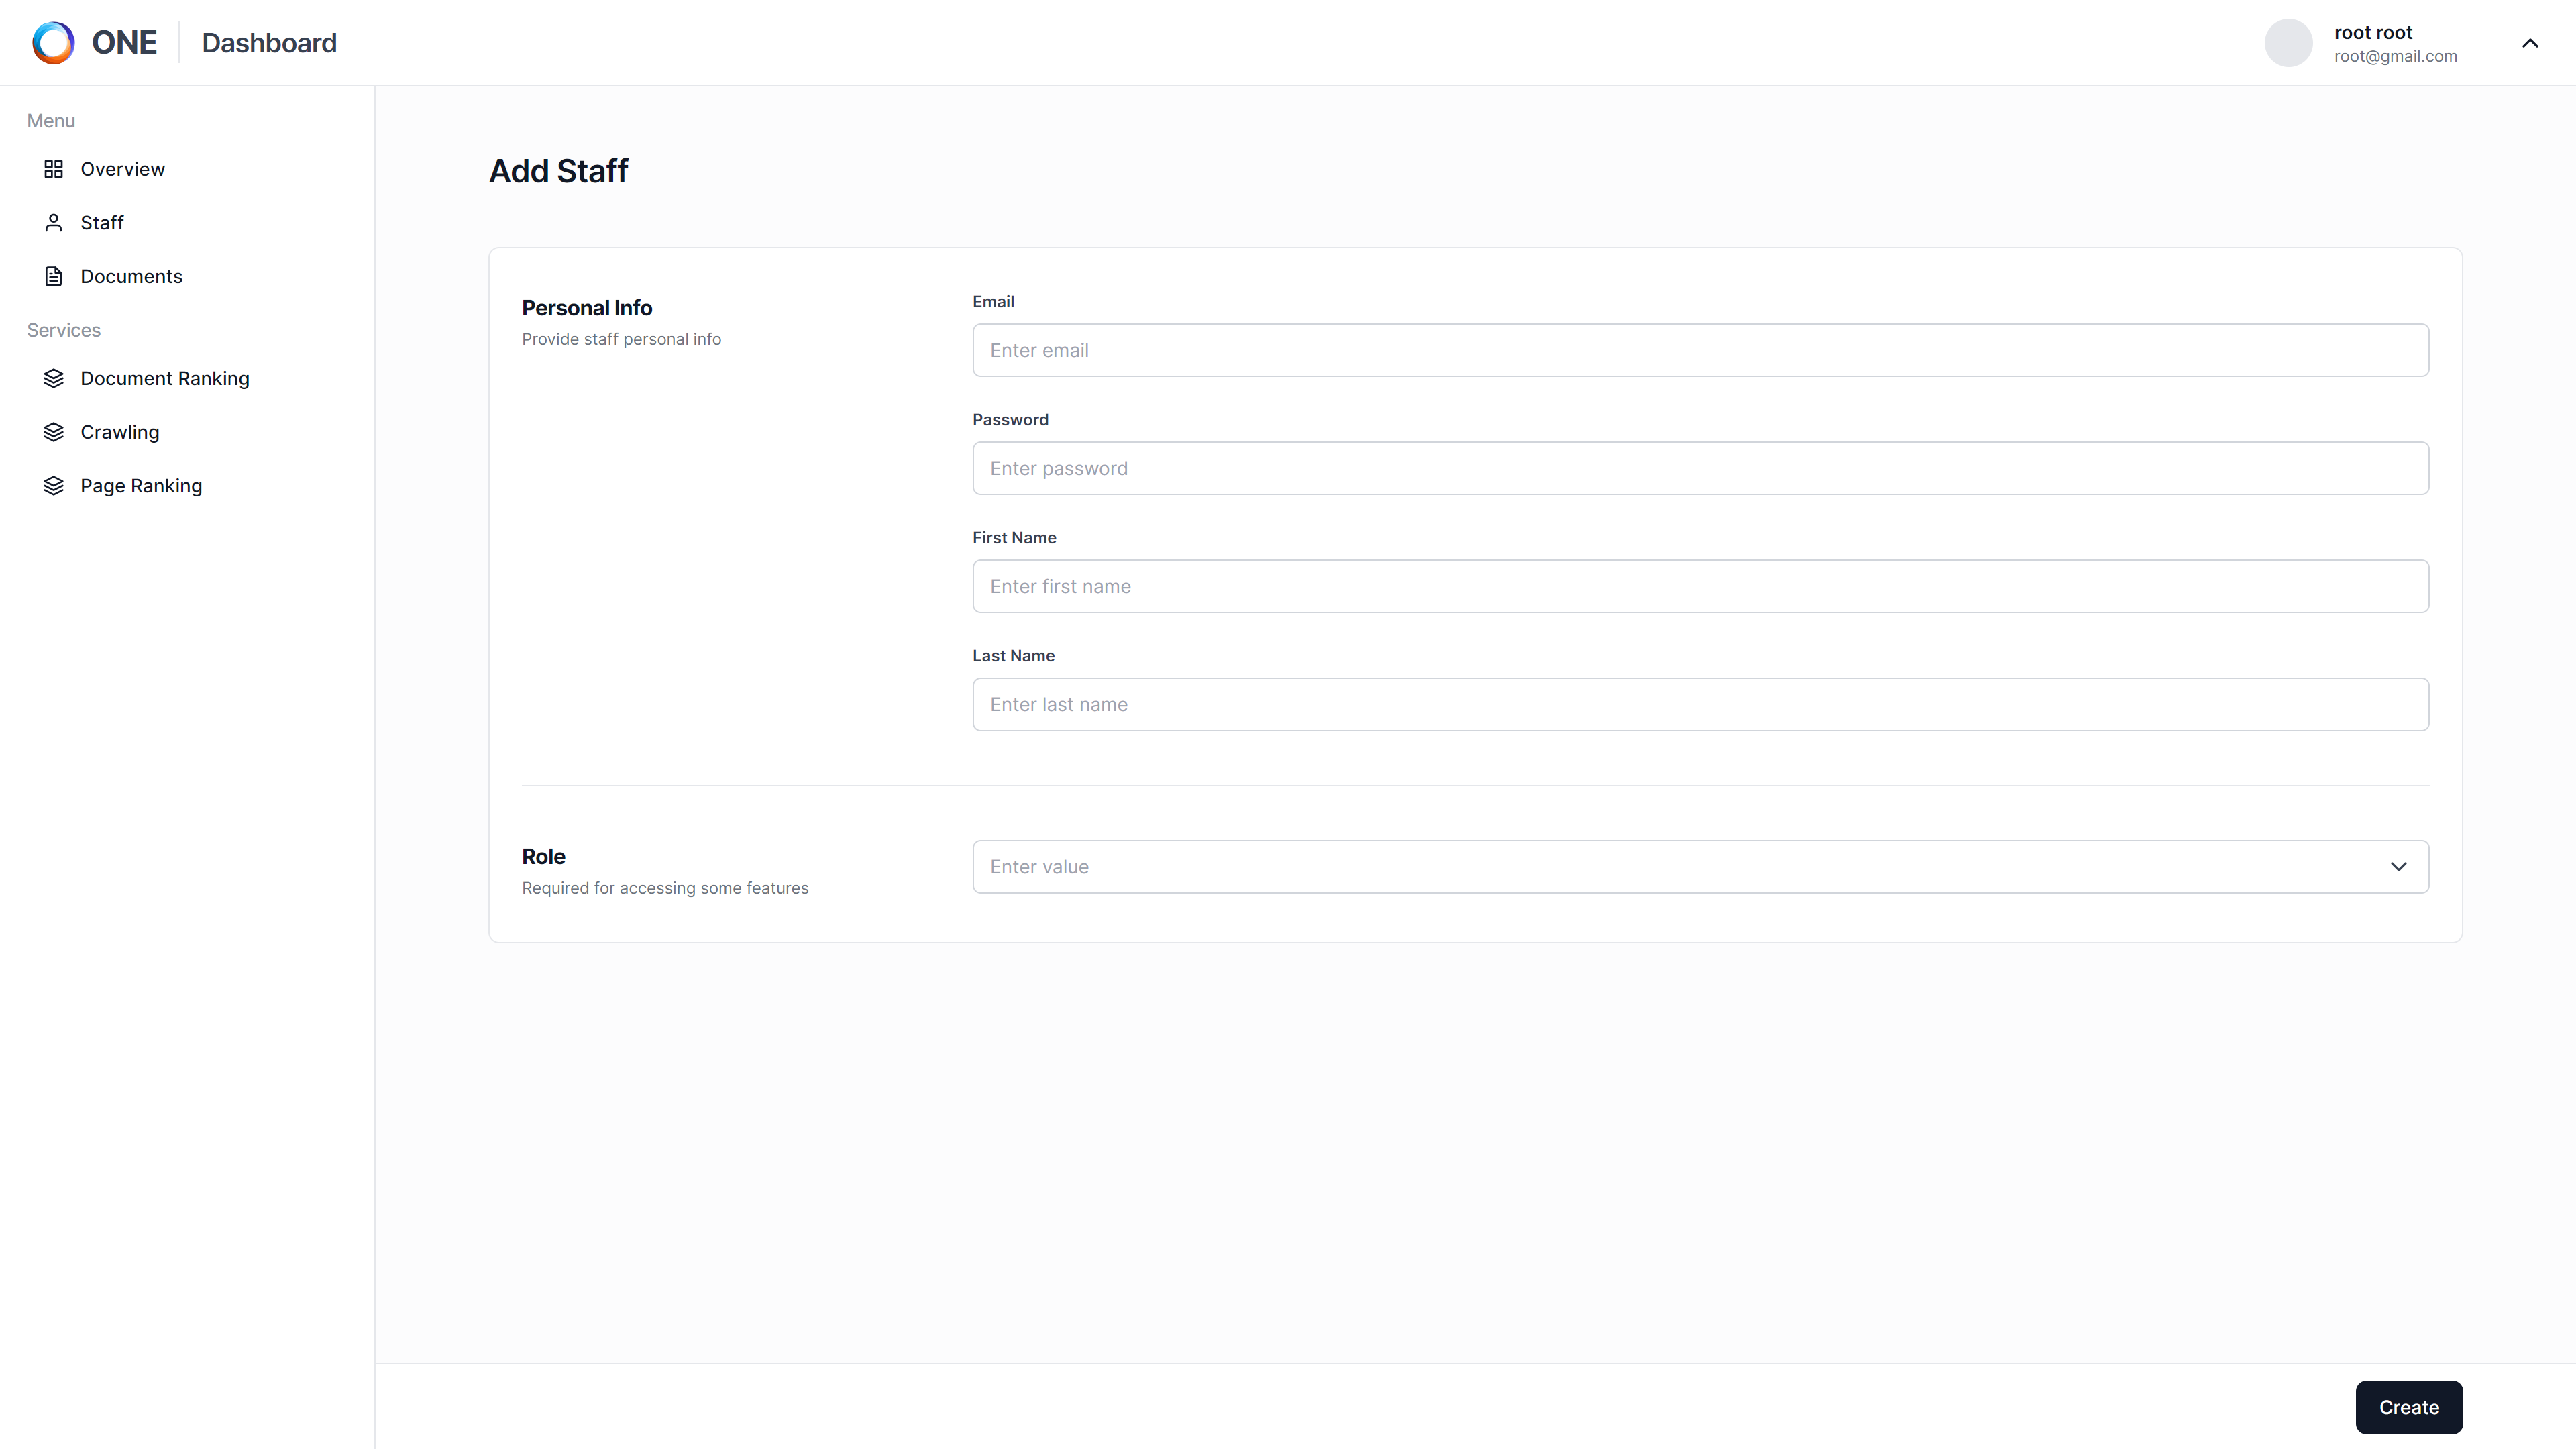
\includegraphics[width=\linewidth]{view_staff_add.png}
	\caption{Halaman tambah \textit{staff}}
	\label{gambar:staff_add}
\end{figure}
\begin{figure}[H]
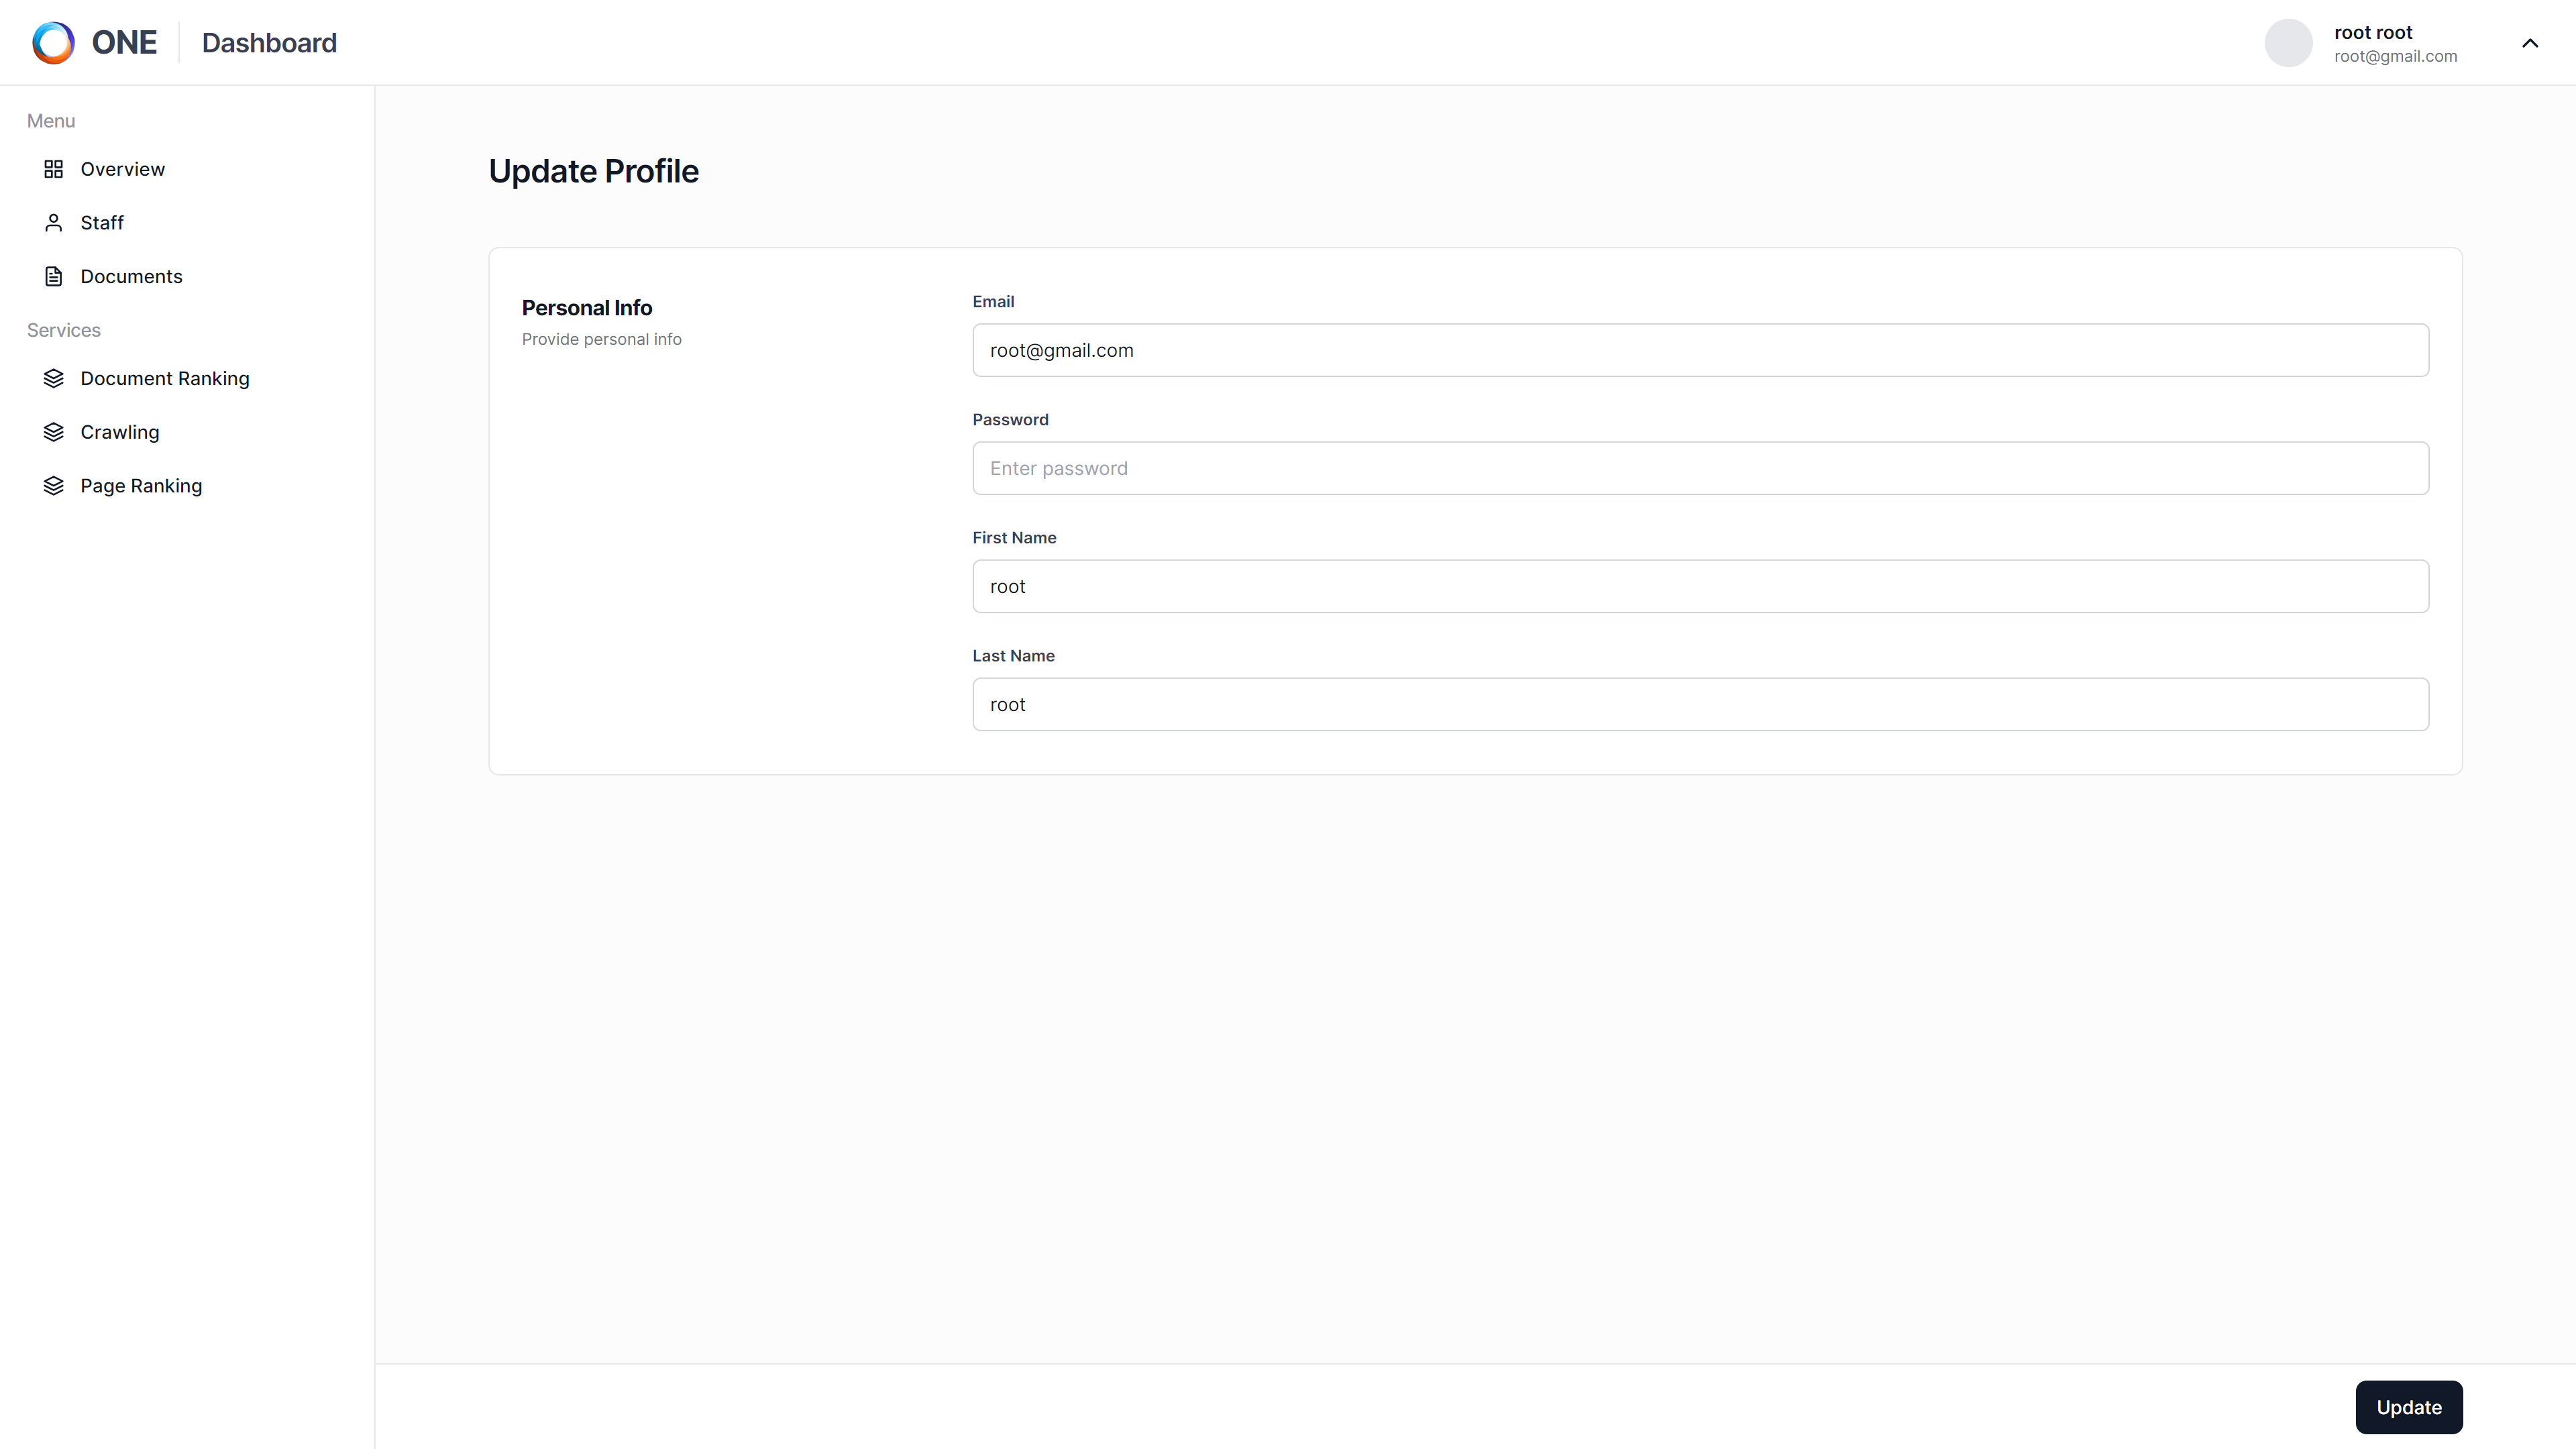
\includegraphics[width=\linewidth]{view_staff_edit.png}
\caption{Halaman ubah \textit{profile}}
\label{gambar:staff_edit}
\end{figure}
\begin{figure}[H]
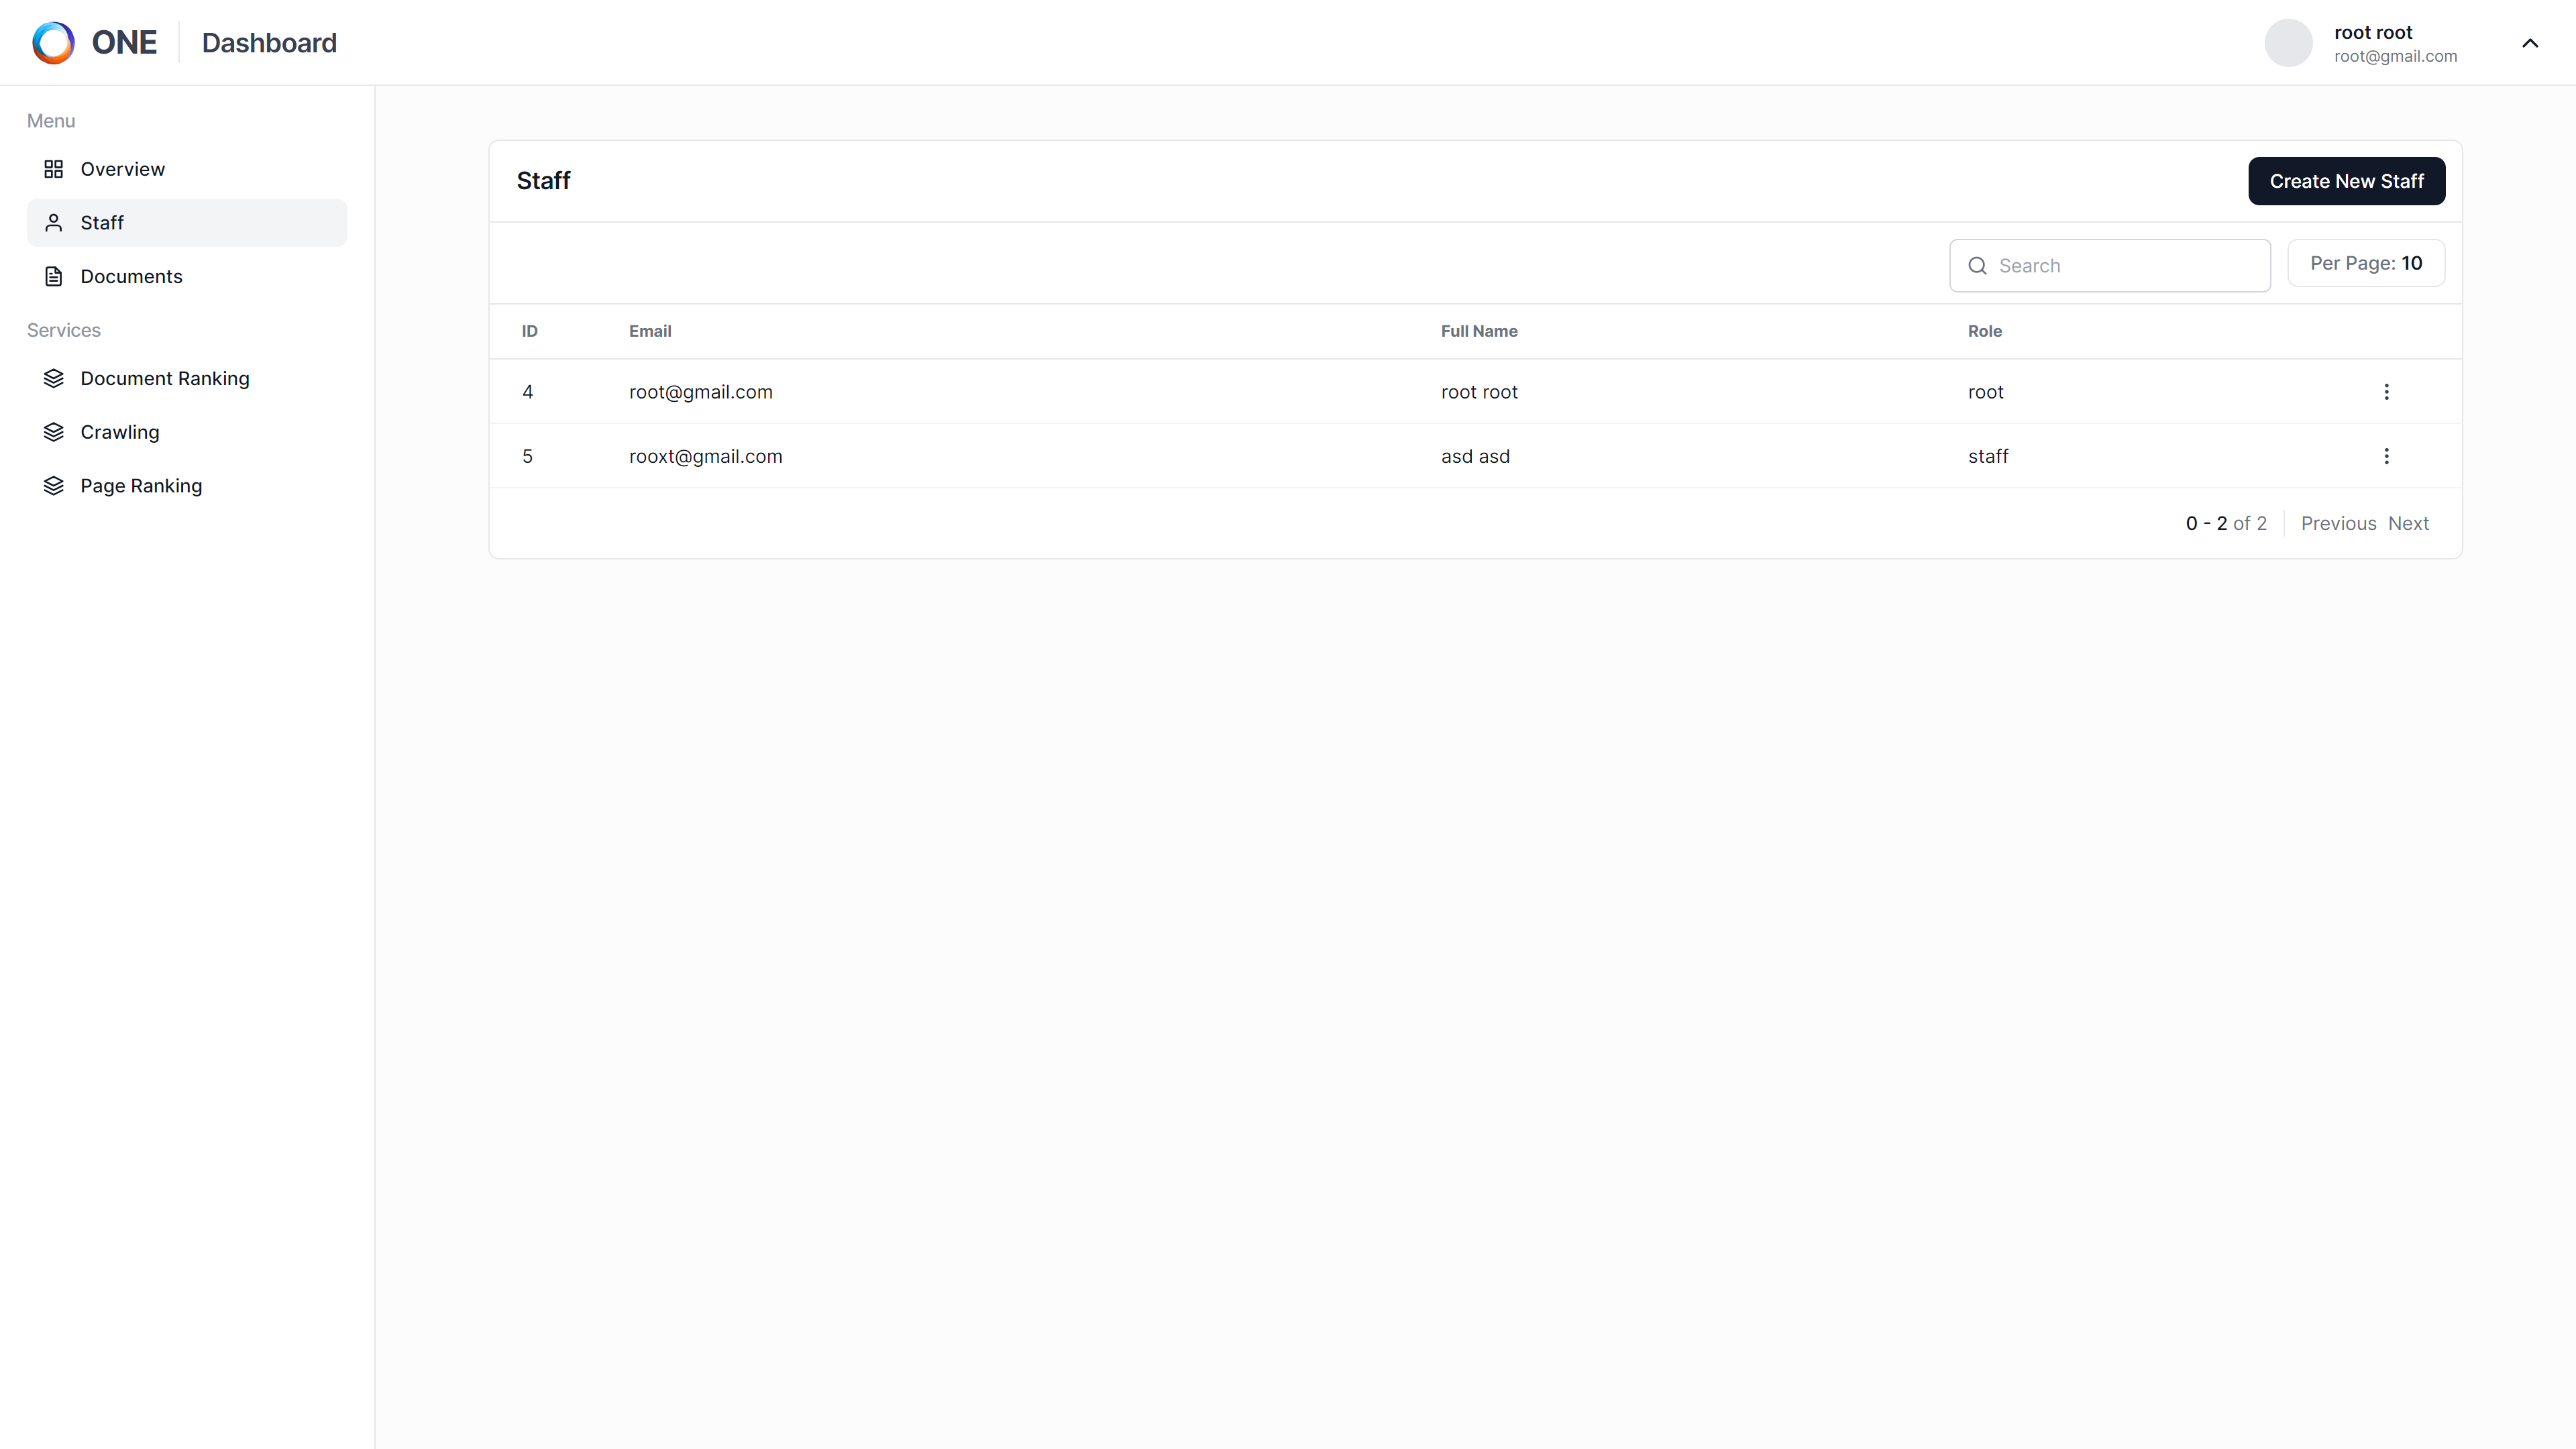
\includegraphics[width=\linewidth]{view_staff_list.png}
\caption{Halaman daftar \textit{staff}}
\label{gambar:staff_list}
\end{figure}
\begin{figure}[H]
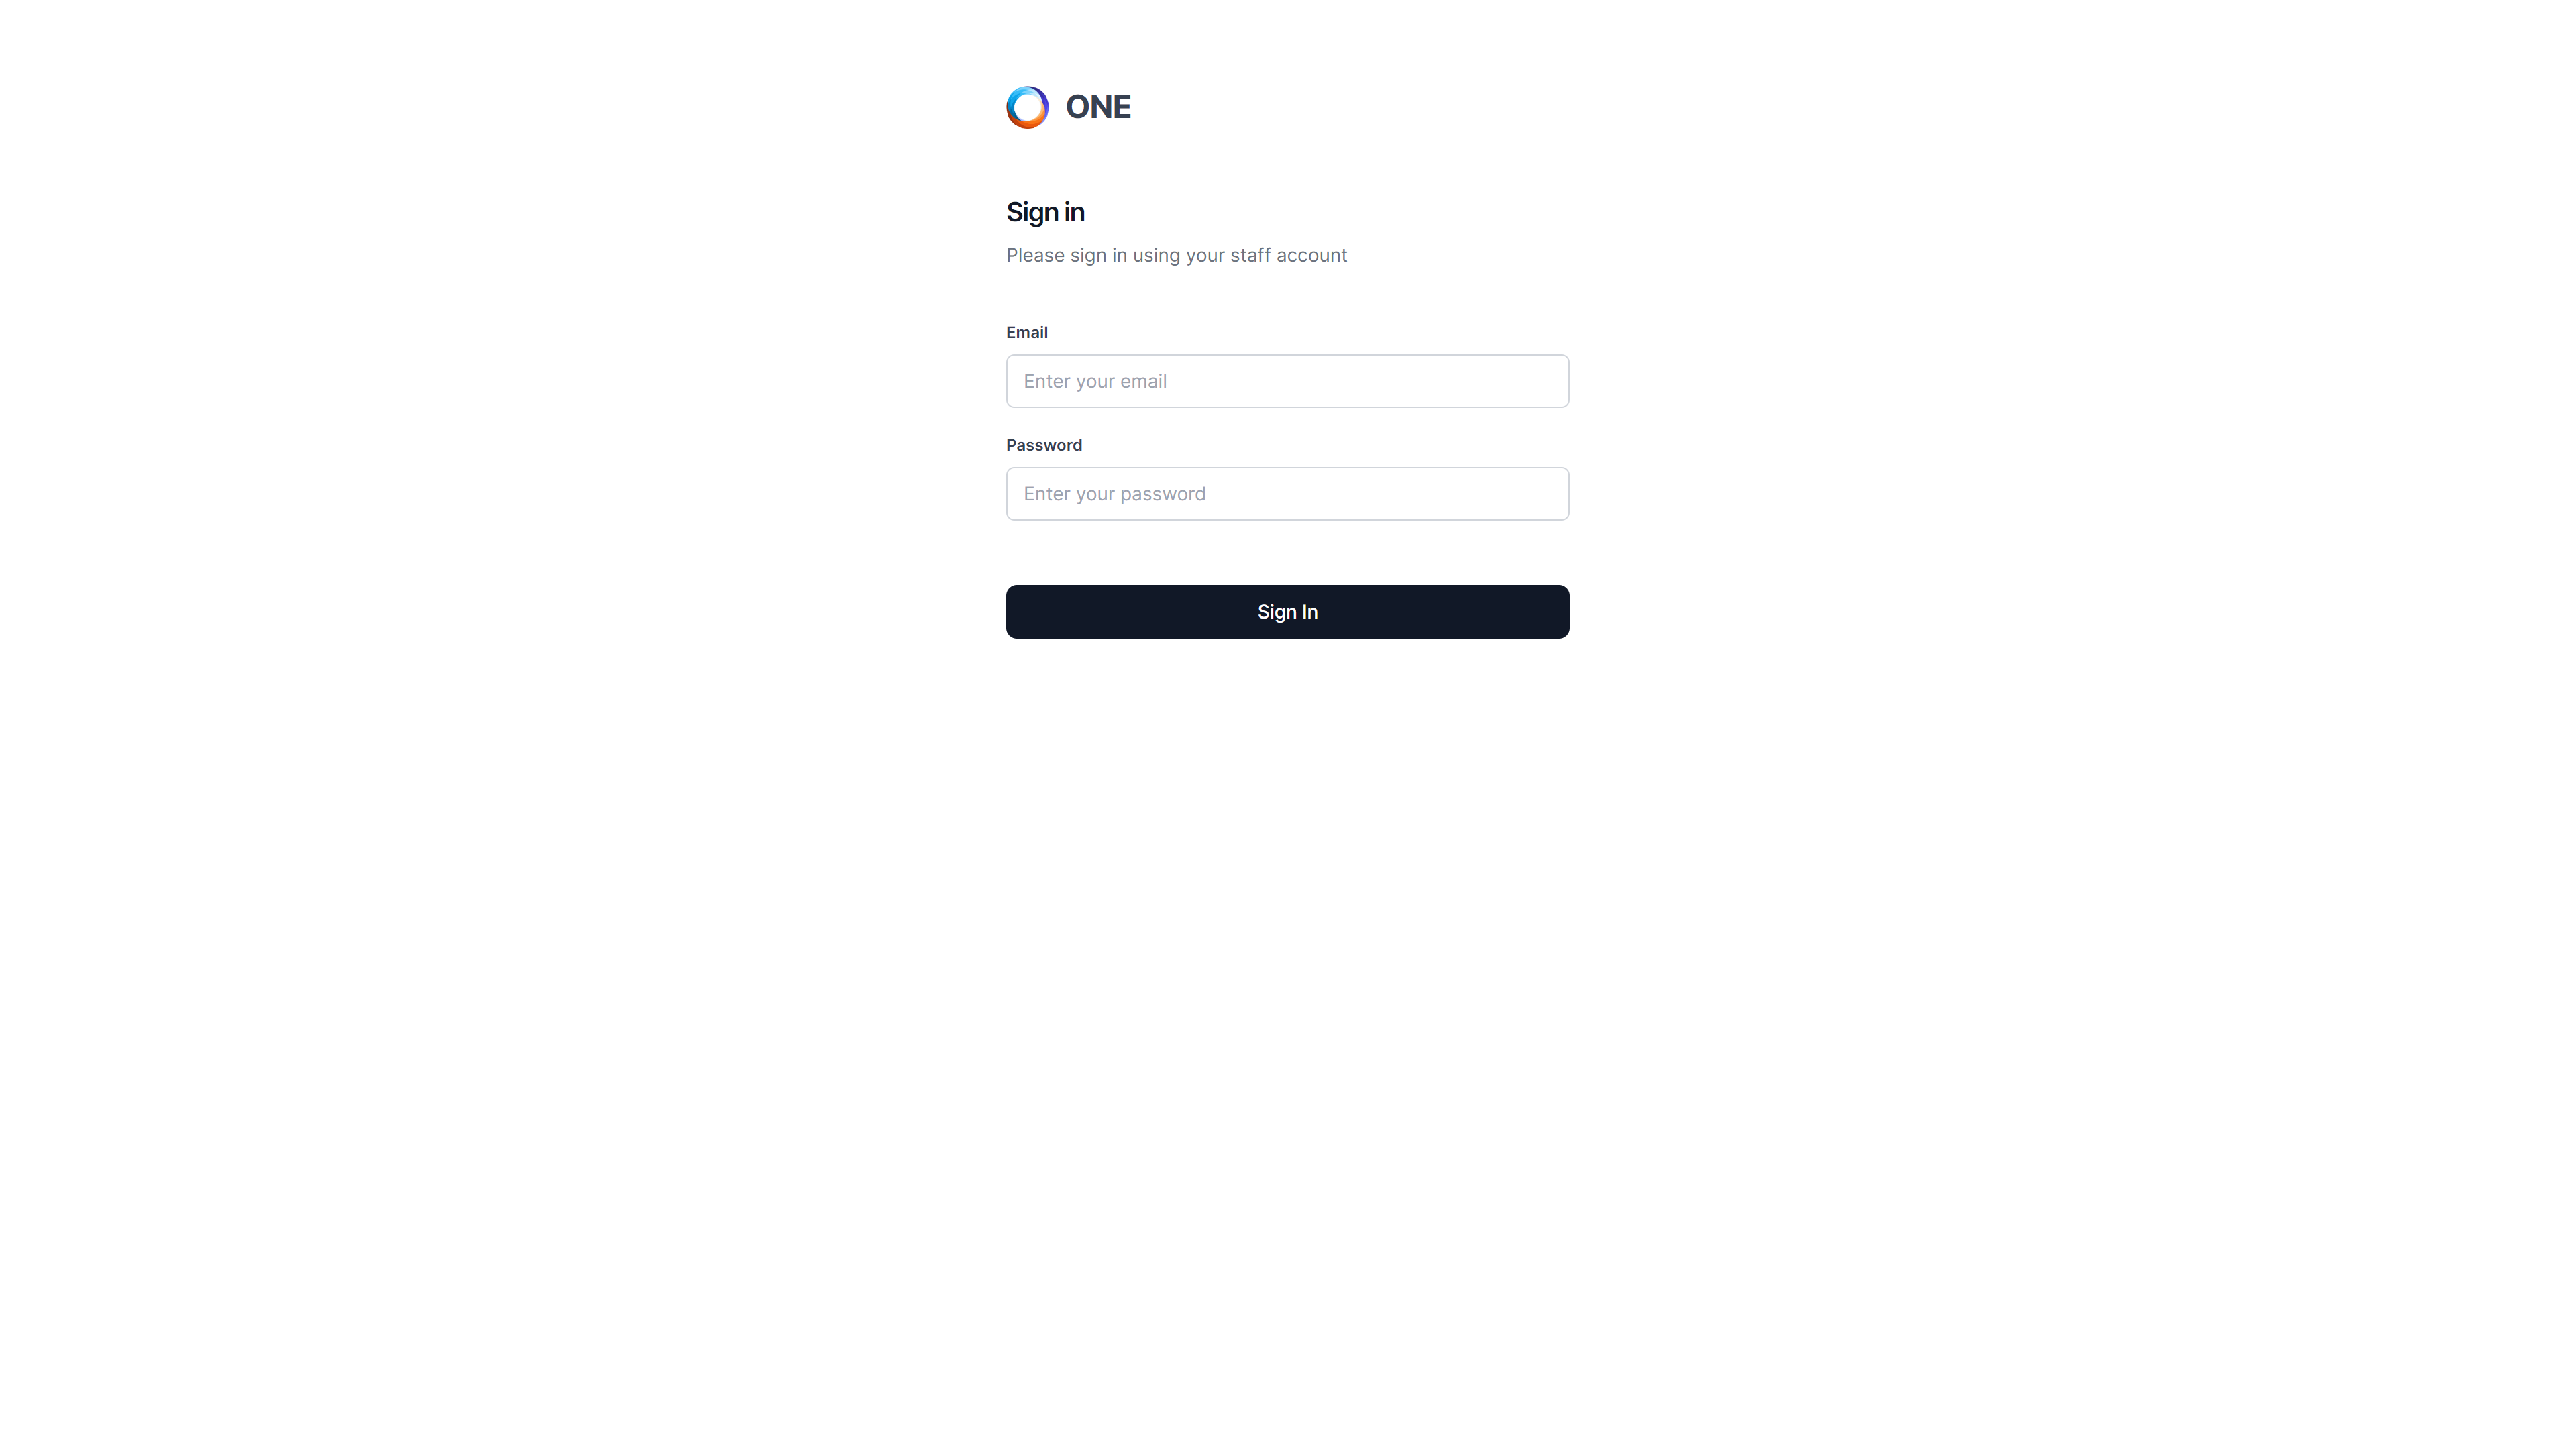
\includegraphics[width=\linewidth]{view_staff_login.png}
\caption{Halaman \textit{login staff}}
\label{gambar:staff_login}
\end{figure}

\subsection{Infrastruktur}
Aplikasi Apache memiliki untuk meneruskan permintaan dari internet publik ke aplikasi web yang terdapat dalam Server yaitu aplikasi web berbasis Flask dengan bahasa pemrograman Python. Aplikasi web berbasis flask ini menangani seluruh permintaan yang datang dari pengguna dan mengirim respon yang sesuai dengan permintaan pengguna. Saat menjalankan tugasnya, aplikasi berbasis flask ini didampingi oleh beberapa aplikasi lainnya yaitu Celery dan MySQL. Aplikasi Celery digunakan oleh aplikasi web berbasis Flask untuk memindahkan sebagian beban kerja yang besar dari aplikasi web berbasis flask yang ada. Dengan adanya pemindahan beban dari aplikasi web berbasis flask ke aplikasi Celery ini, aplikasi web berbasis flask dapat melayani banyak permintaan pengguna yang masuk. Dalam menjalankan tugasnya, aplikasi Celery dibantu oleh aplikasi RabbitMQ yang bertugas sebagai \textit{message broker}. Aplikasi MySQL merupakan aplikasi basis data yang digunakan dalam aplikasi web berbasis Flask. Aplikasi MySQL digunakan untuk menyimpan informasi dan mengambil data yang digunakan oleh aplikasi berbasis Flask.


\begin{figure}[H]
	\centering
	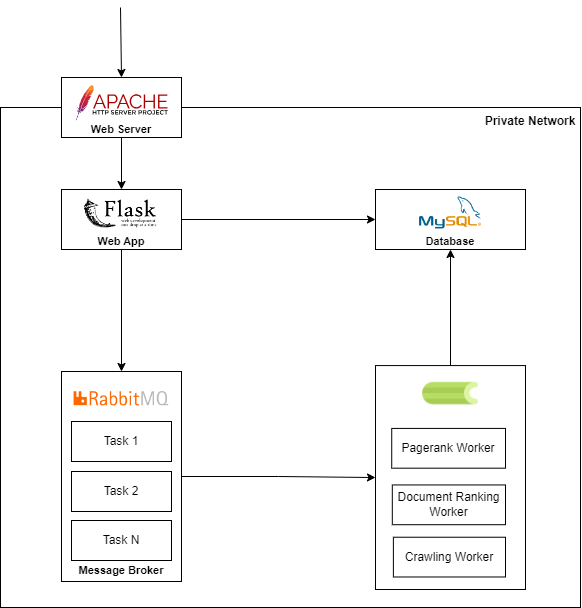
\includegraphics[width=\linewidth]{infra2.png}
	\caption{Infrastruktur \textit{search engine}}
\end{figure}

\subsection{\textit{Memory Profiling}}
Dilakukan pengujian penggunaan memori pada aplikasi \textit{search engine}. Pengujian dilakukan dengan menggunakan pustaka \textit{tracemalloc} dan \textit{gc} dari bahasa pemrograman \textit{python}. Pencacatan penggunaan memori aplikasi dilakukan setiap 30 menit dalam waktu lebih dari satu hari di lingkungan \textit{server}. Pencatatan penggunaan memori dilakukan di dalam spesifikasi perangkat sebagai berikut: 

\begin{enumerate}
	\item 3 \textit{Gigabyte} RAM 
	\item AMD CPU dengan 3 buah \textit{thread}
\end{enumerate}

Adapun grafik penggunaan memori aplikasi adalah sebagai berikut.


\begin{figure}[H]
	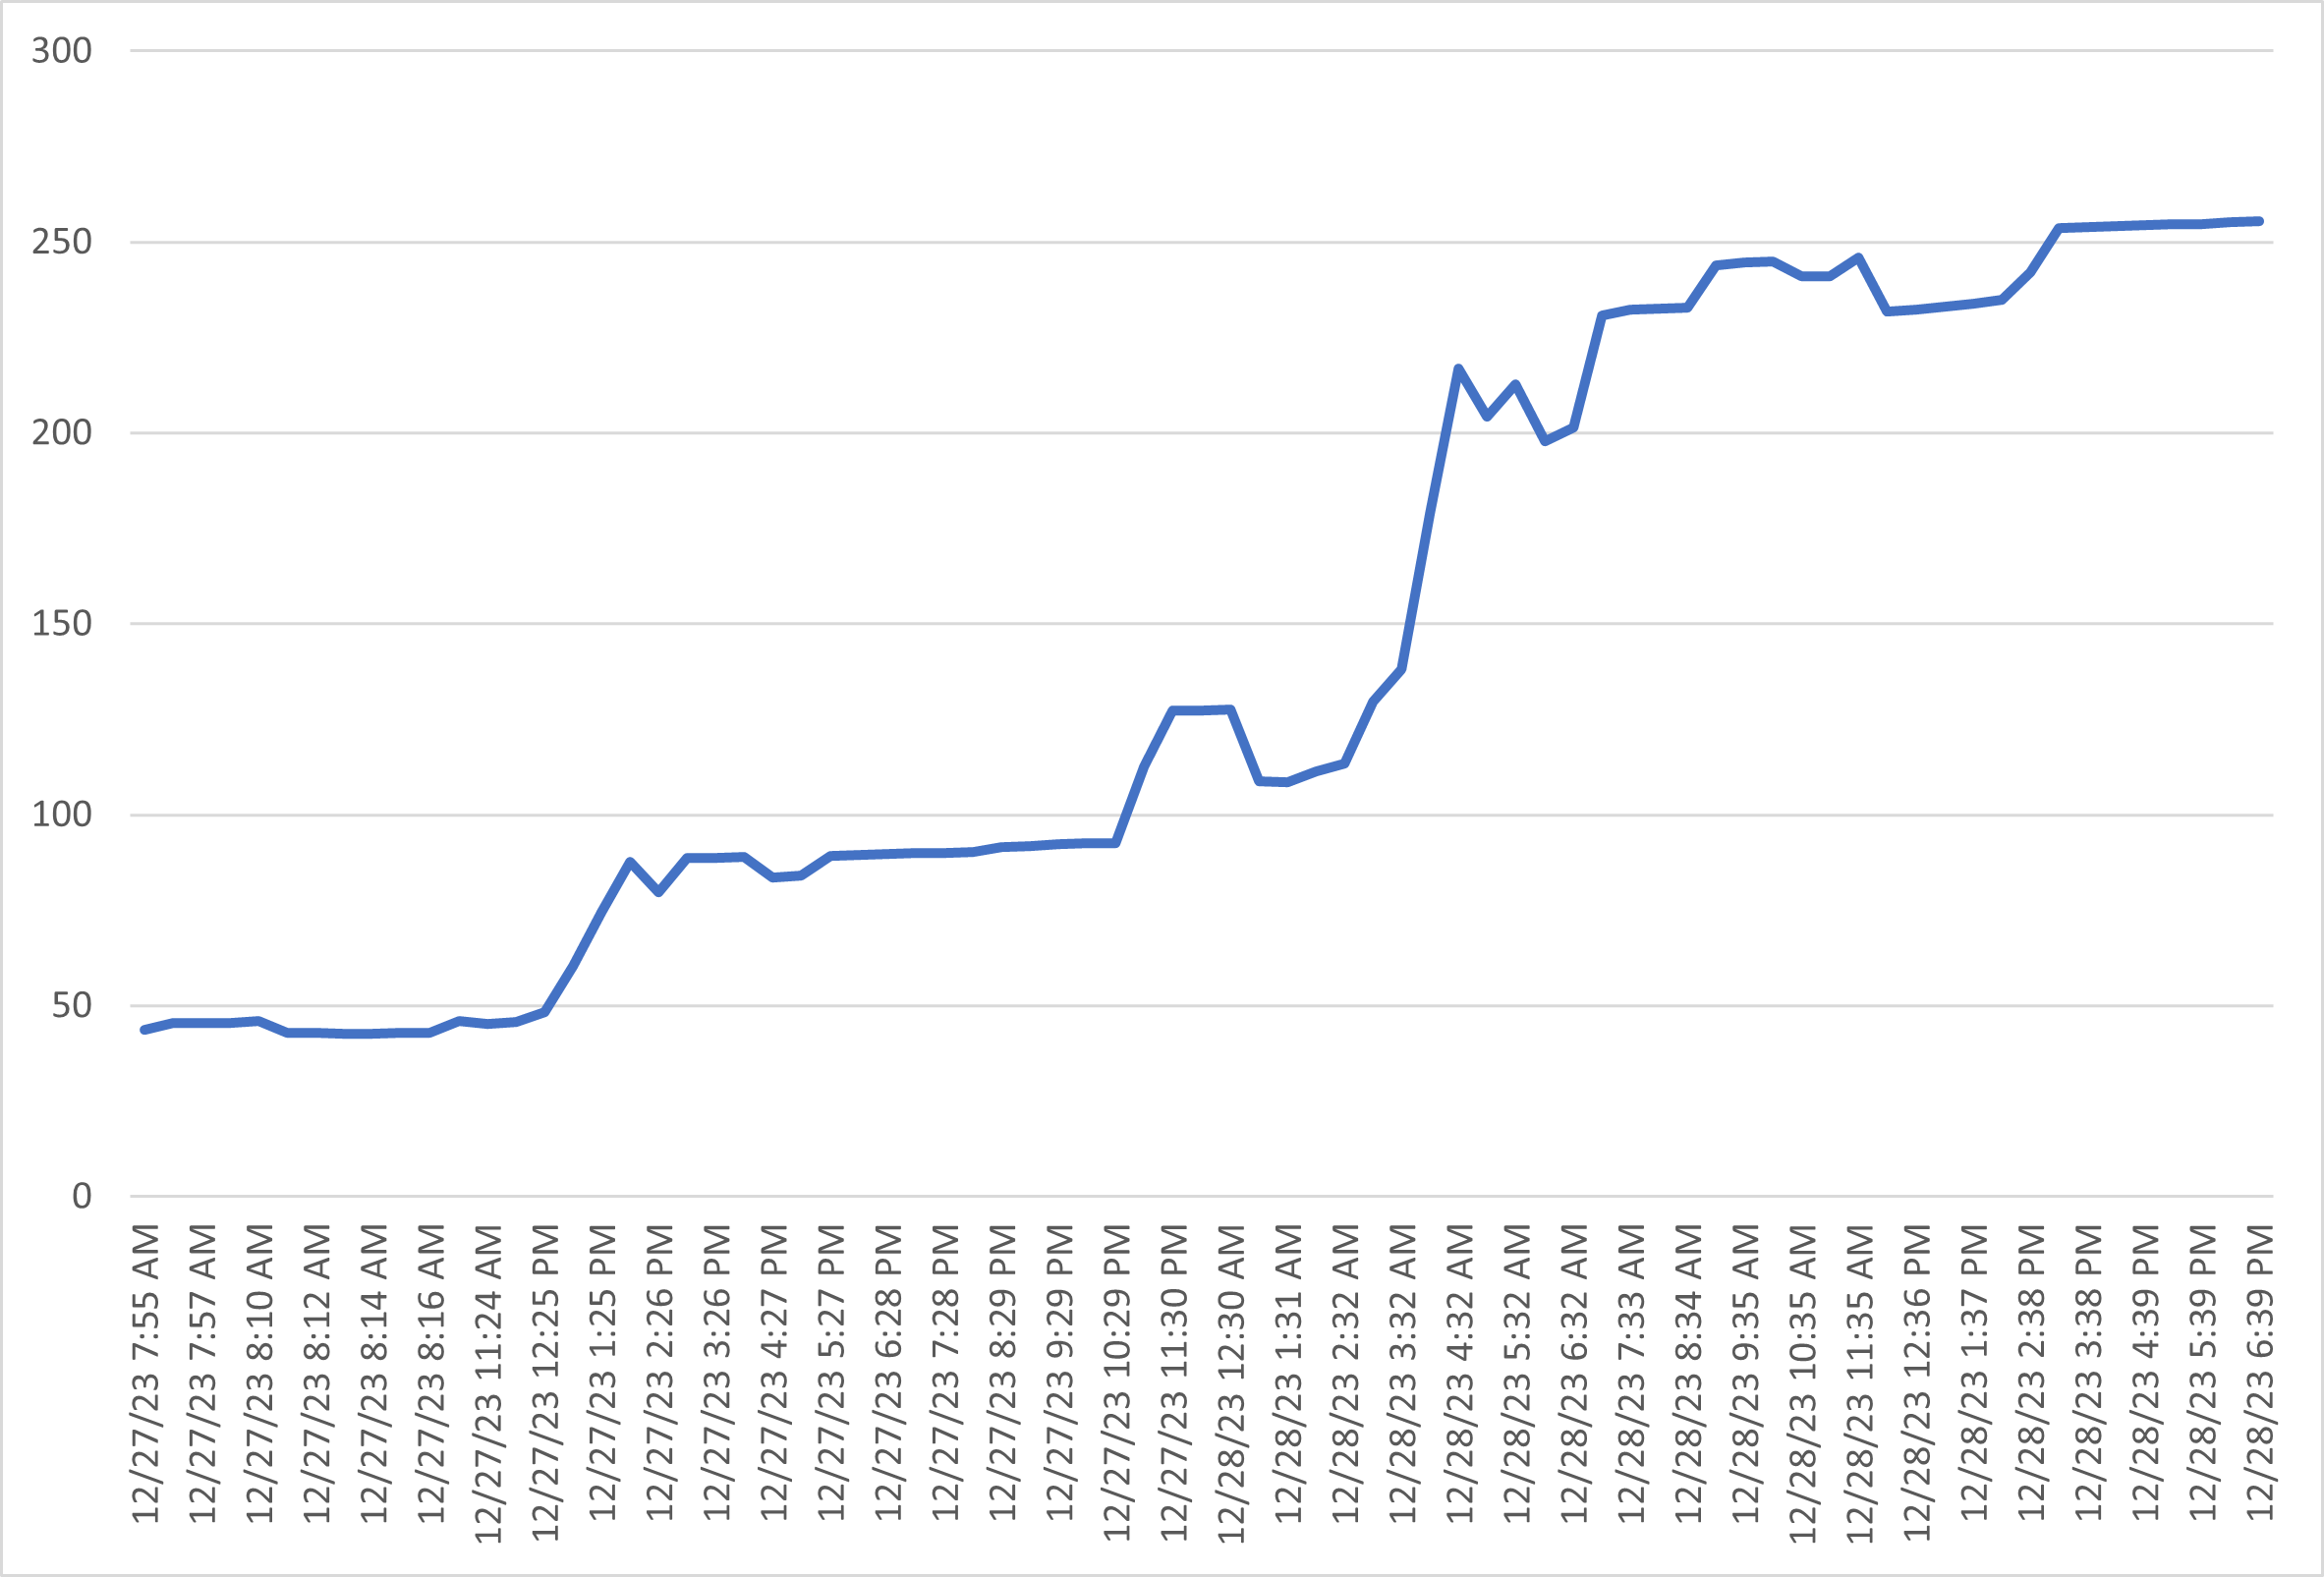
\includegraphics[width=\linewidth]{memchart.png}
	\caption{Grafik penggunaan memori aplikasi \textit{search engine}}
\end{figure}


Percobaan lain dilakukan dengan waktu yang lebih singkat untuk mengidentifikasi letak kenaikan penggunaan memori oleh aplikasi. Dari percobaan yang dilakukan, terdapat kenaikan penggunaan memori yang signifikan dari pustaka \textit{urllib} yang berasal dari bahasa pemrograman \textit{python}. Dari gambar \ref{gambar:linemem}, Dapat disimpulkan kenaikan penggunaan memori terbanyak dari aplikasi disebabkan oleh pustaka dari bahasa pemrograman \textit{python} yang digunakan. Selain itu, untuk peringkat kedua dan ketiga dalam hal penggunaan memori terbanyak berasal dari implementasi algoritma \textit{breadth first search} dari \textit{search engine} pada penelitian \cite{lazu}.

\begin{figure}[H]
	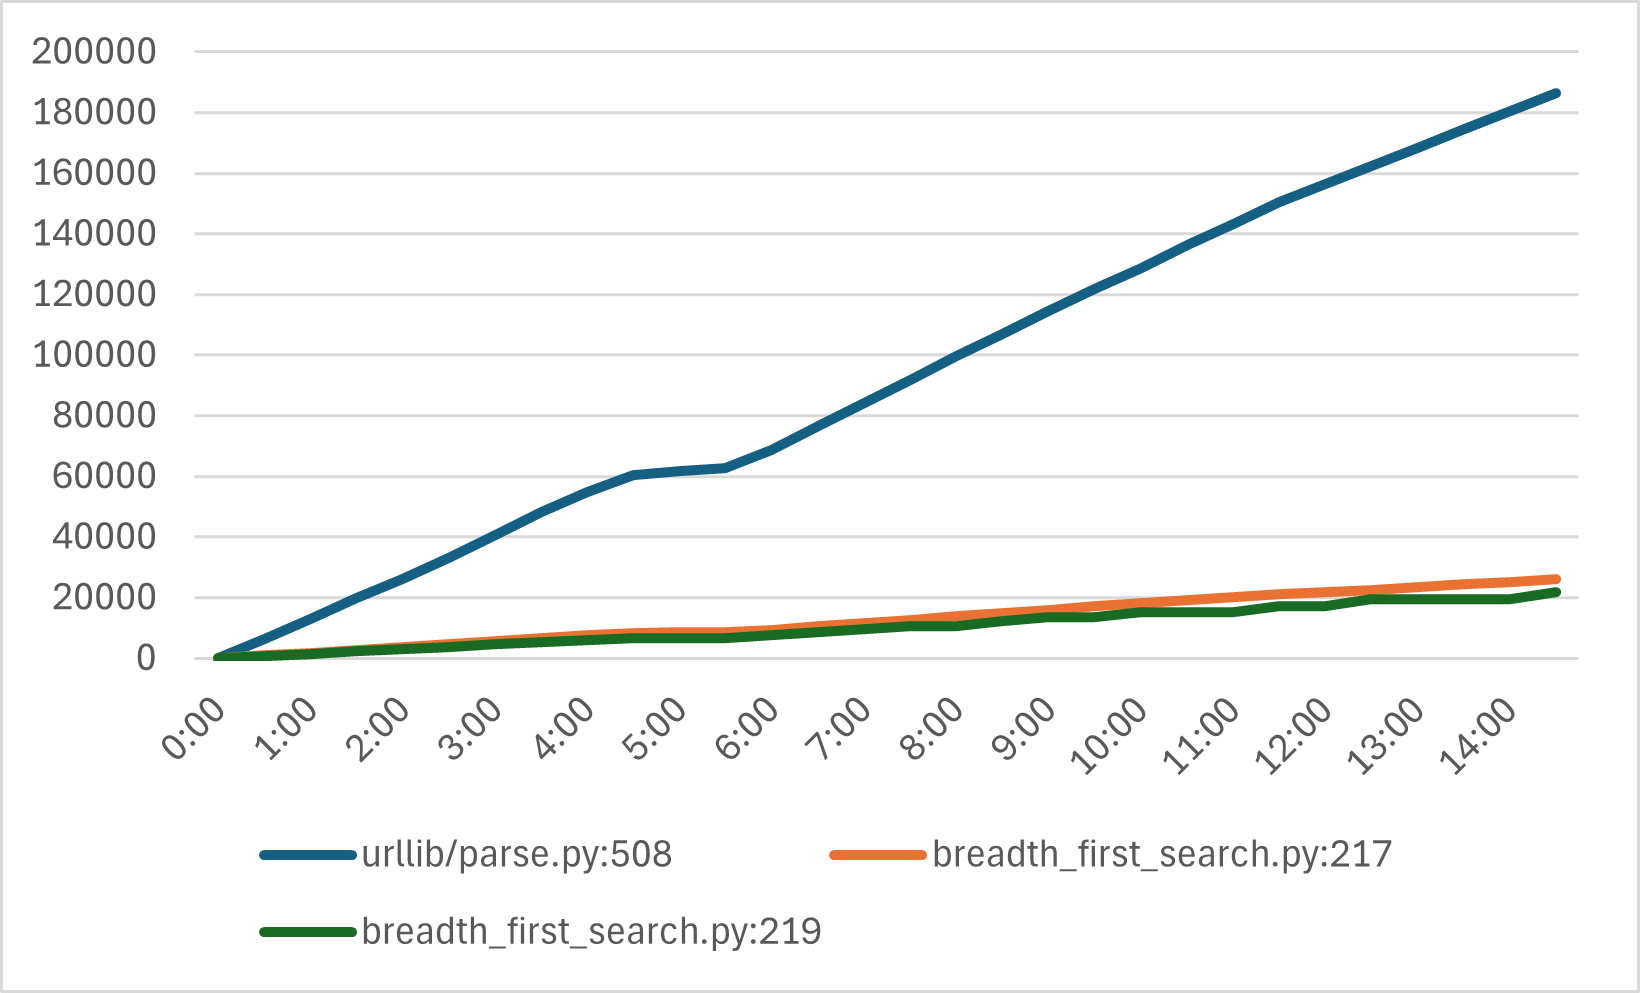
\includegraphics[width=\linewidth]{line_memusage_chart.png}
	\caption{Grafik penggunaan memori terbanyak tiga baris kode aplikasi teratas}
	\label{gambar:linemem}
\end{figure}

\subsection{\textit{Unit Testing}}

Pengujian \textit{unit testing} dilaksanakan dengan salah satu tim pengembang \textit{backend} internal pada saat akhir \textit{sprint}. Kesimpulan dari unit testing yang telah dilakukan adalah fitur yang telah dibuat dapat berjalan dengan baik.

\begin{supertabular}{@{}|p{2cm}|p{2cm}|p{1cm}|p{1.5cm}|@{}}
	\caption{Hasil \textit{Unit Testing}} \\
	\hline
	\multicolumn{4}{|c|}{\textbf{Unit Testing}} \\
	\hline
	&&\multicolumn{2}{c|}{Kesesuaian}\\
	\cline{3-4}
	\textbf{Uji Fitur} & \textbf{Skenario Pengujian} & Sesuai & Tidak Sesuai  \\
	\hline
	Pencarian Pengguna & Pada tampilan halaman pencarian, ketika pengguna memasukkan kata kunci pencarian dan menekan tombol \textit{enter} maka pengguna akan dialihkan ke halaman hasil pencarian & \checkmark & \\
	\hline
	Hasil Pencarian & Saat menekan \textit{tab} peta situs atau \textit{sitemap} maka akan ditampilkan peta situs dari kata kunci yang sedang dicari  & \checkmark &\\
	\cline{2-4} 
	& Pengguna dapat memasukkan kata kunci pencarian dengan memasukkan \textit{query} dengan kunci \textit{search} untuk mendapatkan hasil pencarian & \checkmark & \\
	\hline
	Peta Situs & Pengguna dapat memasukkan kata kunci ulang dengan memasukkan kata kunci pada \textit{text field} di pojok kanan atas lalu menekan tombol \textit{enter} & \checkmark & \\
	\cline{2-4}
	& Pengguna dapat mem-\textit{filter} peta situs berdasarkan negara dengan memilih negara pada tombol \textit{Select Countries} di pojok kanan atas  & \checkmark &\\
	\cline{2-4}
	& Pengguna dapat memasukkan kata kunci pencarian dengan memasukkan kata kunci pencarian pada \textit{query} URL dengan kunci \textit{query} dan negara dengan kunci \textit{countries} & \checkmark &\\
	\hline
	Login & Ketika pengguna memasukkan informasi akun dengan benar ke dalam formulir yang ada maka pengguna akan dialihkan ke halaman \textit{dashboard} & \checkmark &\\
	\cline{2-4}
	& Ketika pengguna memasukkan informasi akun dengan salah ke dalam formulir yang ada maka pengguna akan diberi pesan bahwa pengguna memasukkan informasi akun yang salah &\checkmark&\\	
	\hline
	Dashboard & Ketika pengguna menekan tombol \textit{profile} maka pengguna akan disajikan \textit{popup} yang berisi aksi \textit{logout} & \checkmark&\\
	\hline
	Page Ranking & Ketika pengguna menekan tombol \textit{start}, maka \textit{status page ranking} akan berubah menjadi \textit{running} dan akan muncul tombol \textit{stop} &\checkmark& \\
	\cline{2-4}	
	& Ketika pengguna menekan tombol \textit{stop}, maka \textit{page ranking} akan berhenti dan tombol \textit{start} akan muncul &\checkmark& \\
	\hline
	Crawling & Ketika pengguna menekan tombol \textit{start}, maka \textit{status crawling} akan berubah menjadi \textit{running} dan akan muncul tombol \textit{stop} &\checkmark&  \\
	\cline{2-4}
	& Ketika pengguna menekan tombol \textit{stop}, maka \textit{crawling} akan berhenti dan tombol \textit{start} akan muncul &\checkmark& \\
	\cline{2-4}
	& Saat \textit{tab} \textit{domains} diklik, pengguna akan dialihkan ke sub halaman daftar domain &\checkmark& \\
	\cline{2-4}
	& Saat \textit{tab} \textit{webpages} diklik, pengguna akan dialihkan ke sub halaman daftar \textit{webpages} &\checkmark& \\
	\hline
	Daftar Situs & Ketika pengguna menekan salah satu situs pada daftar situs, pengguna akan dialihkan ke halaman detail situs &\checkmark& \\
	\hline
	& Pengguna dapat menyaring daftar \textit{situs} yang dimunculkan dengan mengaplikasikan \textit{filter} yang tersedia yang terletak di atas tabel &\checkmark& \\
	Daftar \textit{Domain} & Pengguna dapat menyaring daftar \textit{domain} yang dimunculkan dengan mengaplikasikan \textit{filter} yang tersedia yang terletak di atas tabel &\checkmark& \\
	\cline{2-4}
	\textit{Document Ranking} & Ketika pengguna menekan tombol \textit{start}, maka \textit{status document ranking} akan berubah menjadi \textit{running} dan akan muncul tombol \textit{stop}&\checkmark&  \\
	\cline{2-4}
	& Ketika pengguna menekan tombol \textit{stop}, maka \textit{document ranking} akan berhenti dan tombol \textit{start} akan muncul &\checkmark& \\
	\cline{2-4}
	& Ketika pengguna menekan \textit{tab} \textit{words}, maka akan dialihkan ke sub halaman \textit{words} &\checkmark& \\
	\cline{2-4}		
	& Ketika pengguna menekan \textit{tab} \textit{search log}, maka akan dialihkan ke sub halaman \textit{search log} &\checkmark& \\
	\hline
	Daftar Staff & Ketika tombol \textit{create new staff} ditekan, maka akan dialihkan ke halaman tambah \textit{staff} baru &\checkmark& \\
	\cline{2-4}
	&  Ketila tombol \textit{more} yang dilambangkan dengan ikon tiga titik vertikal ditekan, maka akan muncul \textit{popup} yang berisi aksi \textit{delete staff}. &\checkmark& \\
	\cline{2-4}
	& Ketika \textit{delete staff} ditekan, maka \textit{staff} akan dihapus dari daftar \textit{staff} setelah melakukan \textit{refresh} ulang. &\checkmark& \\
	\hline
	Tambah Staff & Ketika form berhasil diisi maka \textit{staff} baru akan ditambahkan ke daftar \textit{staff} &\checkmark& \\
	\hline
\end{supertabular}


\section{Kesimpulan}
Berdasarkan  hasil  implementasi  dan  pengujian  pada program ini, maka didapatkan kesimpulan sebagai berikut:
\begin{enumerate}
	\item Perancangan aplikasi \textit{admin console} untuk manajemen dan visualisasi data hasil pengindeksan \textit{search engine} yang telah dibuat pada penelitian \cite{lazu} yang dirancang menggunakan metode \textit{scrum}.
	\item Pada pengujian penggunaan memori aplikasi, diketahui adanya kenaikan penggunaan memori secara signifikan. Dalam pengujian terpisah, dilakukan pengujian untuk menemukan letak baris kode yang menggunakan memori terbanyak yang dapat dilihat pada gambar \ref{gambar:linemem}. Pada peringkat pertama, baris kode yang menggunakan memori terbanyak dan memiliki kenaikan penggunaan memori yang signifikan berasal dari pustaka bawaan bahasa pemrograman python itu sendiri. Selain itu, baris kode peringkat kedua dan ketiga dalam hal penggunaan memori terbanyak berasal dari implementasi \textit{search engine} pada penelitian \cite{lazu}. 
\end{enumerate}


%----------------------------------------------------------------------------------------
%	 REFERENCES
%----------------------------------------------------------------------------------------

\bibliography{sample}
\bibliographystyle{abbrv}


%----------------------------------------------------------------------------------------

\end{document}
